\documentclass{sig-alternate}
\usepackage{color}
\usepackage[colorinlistoftodos]{todonotes}
\usepackage{algorithm}
\usepackage[noend]{algpseudocode}

\newtheorem{theorem}{Theorem}

\algnewcommand\algorithmicinput{\textbf{Input:}}
\algnewcommand\Input{\item[\algorithmicinput]}


%%%%% Uncomment the following line and comment out the previous one
%%%%% to remove all comments
%%%%% NOTE: comments still occupy a line even if invisible;
%%%%% Don't write them as a separate paragraph
%\newcommand{\mycomment}[1]{}

\begin{document}

\conferenceinfo{UMM CSci Senior Seminar Conference, April 2017}{Morris, MN}

\title{Conflict-Free Vertex Coloring Of Planar Graphs}

\numberofauthors{1}

\author{
\alignauthor
Shawn Seymour\\
	\affaddr{Division of Science and Mathematics}\\
	\affaddr{University of Minnesota, Morris}\\
	\affaddr{Morris, Minnesota, USA 56267}\\
	\email{seymo079@morris.umn.edu}
}

\maketitle
\begin{abstract}
The conflict-free coloring problem is a variation of the vertex coloring problem, a classical NP-hard optimization problem. The conflict-free coloring problem aims to color a possibly proper subset of vertices such that there is a unique color within the closed neighborhood (a vertex and its neighbors) of every vertex. This paper presents recent findings and heuristics to solve the conflict-free coloring problem on both general graphs and planar graphs.
\end{abstract}

\section{Introduction}
\label{sec:introduction}

Consider the map of the 48 contiguous states in the United States of America. Suppose we would like to color each state such that no two states that share a boundary have the same color. This problem can be modeled with a graph. We can represent each state with a \emph{vertex} and represent a boundary between two states with an \emph{edge}.

This is a famous example of the \emph{vertex coloring} problem and one of many graph coloring problems. The vertex coloring problem aims to find the minimum number of colors needed to color a graph such that no two adjacent vertices are colored with the same color. While some problems are relatively easy to solve, the vertex coloring problem is one of the most computationally complex problems in computer science and mathematics \cite{bondy1976graph}. The vertex coloring problem has many real-world applications such as finding the minimum number of time slots needed to schedule final exam periods such that no two courses (taken by the same student) are scheduled at the same time slot.

The \emph{conflict-free coloring} problem is a relaxed variation of the vertex coloring problem. The conflict-free coloring problem does not aim to color \emph{every} vertex. Rather, it aims to color \emph{some} vertices such that the neighborhood of every vertex contains at least one uniquely colored vertex.

This paper looks into some applications and heuristics of conflict-free coloring. We then look into the specific case of conflict-free coloring planar graphs. Section 2 provides the background necessary to understand the problem and how it is used. Section 3 introduces some applications for the conflict-free coloring problem. Section 4 describes a heuristic for conflict-free coloring general graphs. Section 5 looks into the specific case of conflict-free coloring planar graphs.


\section{Background}
\label{sec:background}
To understand the problem, the algorithms to solve it, and its results, we must first understand some graph theory, some computational complexity theory, and the precise definitions of the vertex coloring problem and the conflict-free coloring problem.

\begin{figure}[h]
	\centering
	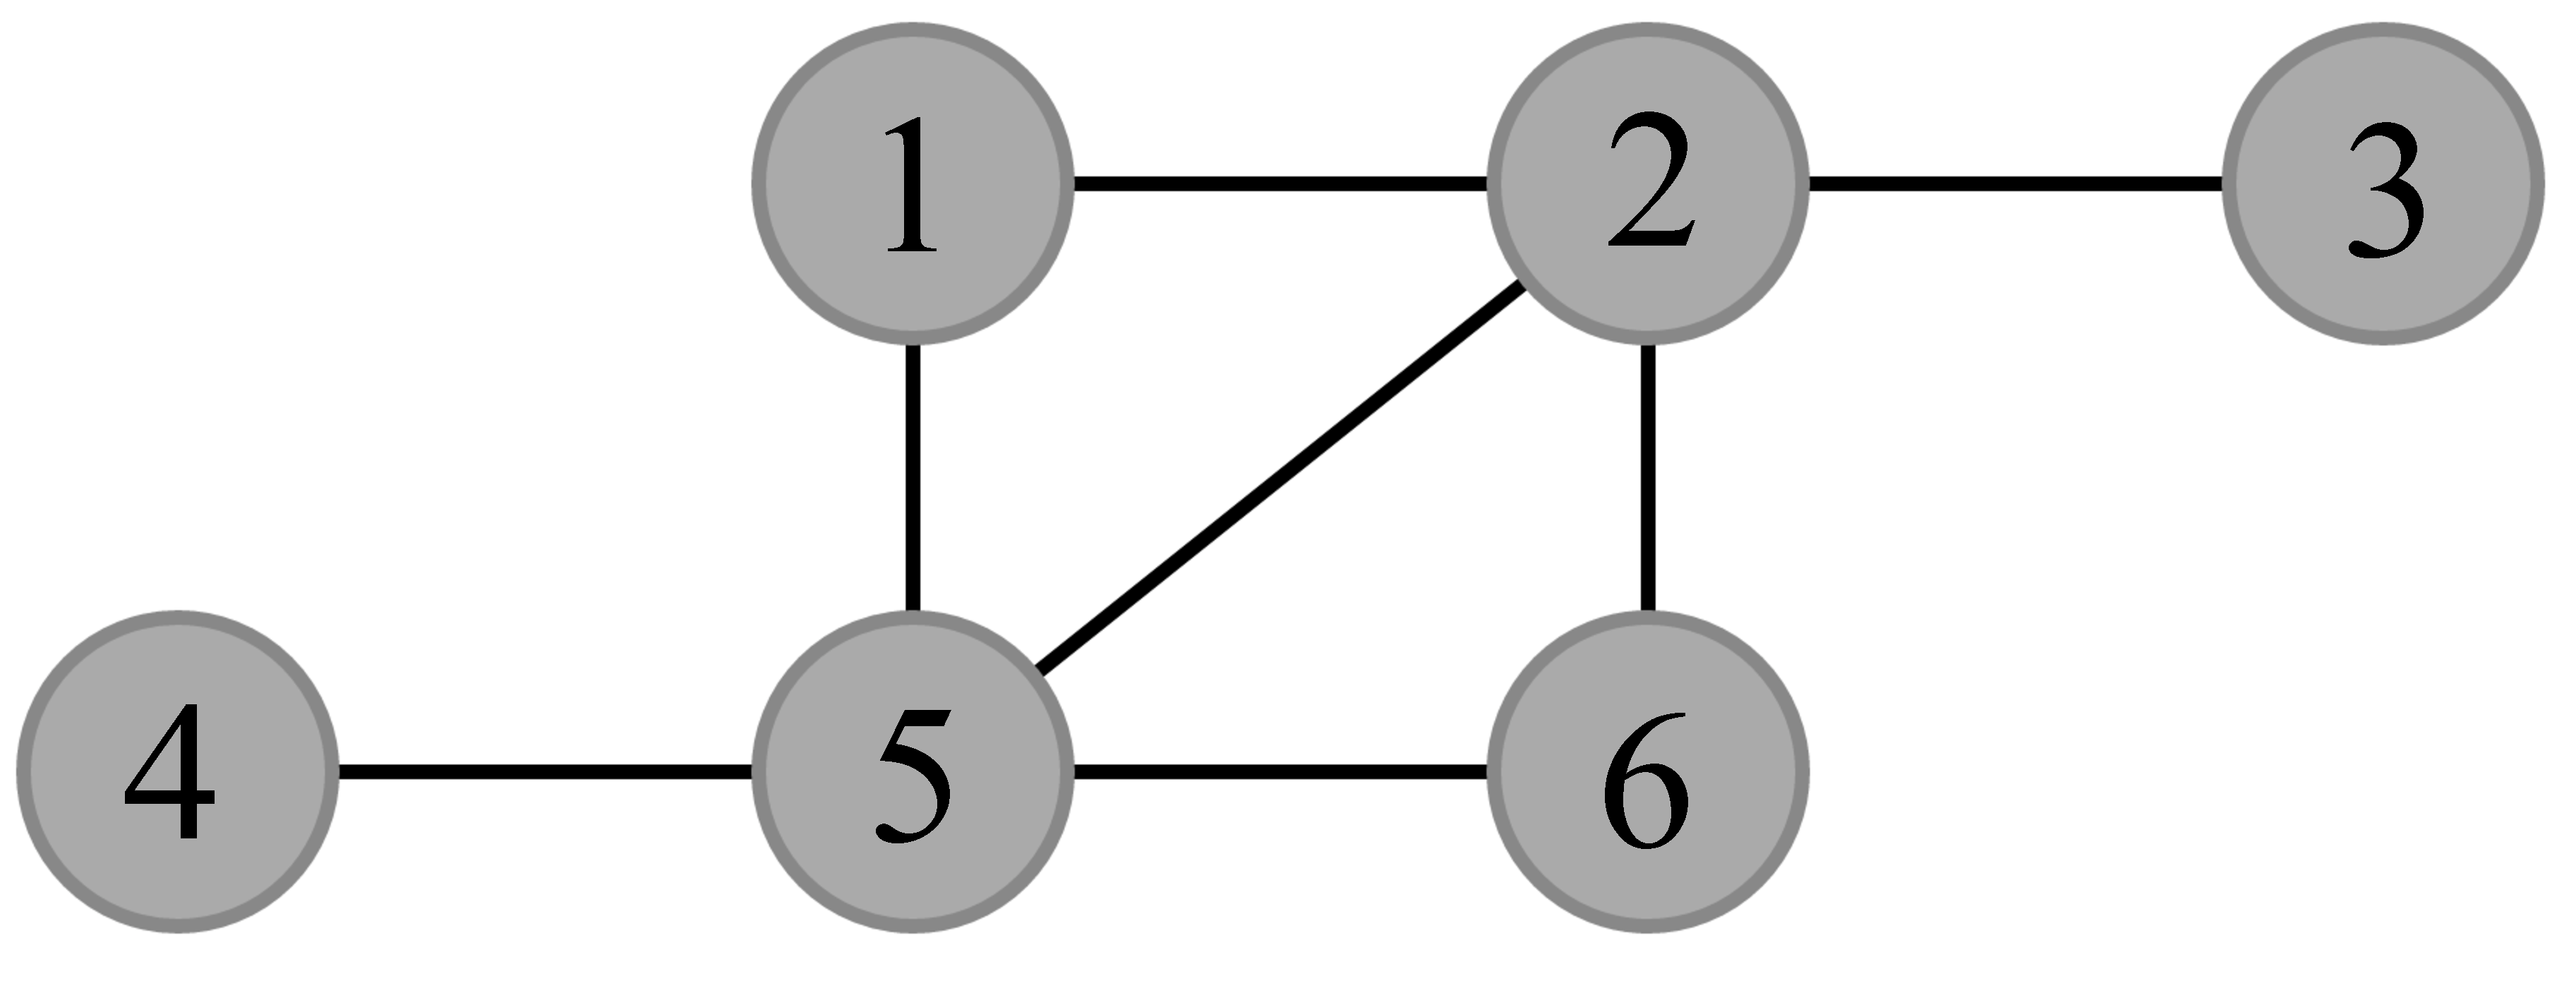
\includegraphics[width=7cm]{../figures/example.pdf}
	\caption{A simple, undirected graph $G_1$}\label{fig:graph}
\end{figure}

\subsection{Graph Theory}
\label{sec:graphtheory}

A graph, denoted $G=(V,E)$, is an ordered pair of two sets: a set of vertices $V$ and a set of edges $E$. Each edge consists of a set of two unordered vertices from $V$. For example, $\{u, w\} \in E$ is an edge connecting vertices $u$ and $w$ where $u,w \in V$. Vertices are \emph{adjacent} if they are connected by an edge. An edge that connects a vertex to itself is called a \emph{loop}. A graph without loops is called \emph{loopless}.

A simple graph is a loopless graph where no two edges connect the same pair of vertices. A planar graph is a graph that can be drawn on the plane such that its edges only intersect at their endpoints. This drawing is referred to as a planar drawing. All graphs used by the vertex coloring problem and conflict-free coloring problem are assumed to be simple graphs. An example graph is shown in Figure \ref{fig:graph}.

The open neighborhood of a vertex is a set of all vertices adjacent to $v$. A \emph{closed} neighborhood, denoted $N_G(v)$, consists of the vertices adjacent to $v$ plus $v$ itself. For example, let's examine $N_{G_1}(1)$ from Figure \ref{fig:graph}. The open neighborhood of 1 is $\{2, 5\}$ while the closed neighborhood is $\{1, 2, 5\}$. For the rest of the paper, the term \emph{neighborhood} will refer to closed neighborhoods unless stated otherwise.

A \emph{path} is a sequence of edges that connect a sequence of distinct vertices. A \emph{subgraph} is a graph $H$ that can be formed from a subset of the vertices and edges of $G$. A graph is \emph{connected} if there exists a path between every pair of vertices. A \emph{component} of a graph $G$ is a subgraph $H$ where $H$ is connected and $H$ is not contained in any connected subgraph of $G$ that has more vertices or edges than $H$ has. An isolated path is a component that is itself a path.

The distance of a path can be thought of as the smallest number of edges needed to get from one vertex to another vertex. For example, in Figure \ref{fig:graph}, the distance from vertex 3 to vertex 4 would be 3 as it takes 3 edges to get there. A \emph{distance-3-set} is a set of vertices that all have exactly pairwise distance 3 from each other. An example of a distance-3-set from Figure \ref{fig:graph} would be $\{3,4\}$. \cite{bondy1976graph,west2001introduction}

\begin{figure}[h]
	\centering
	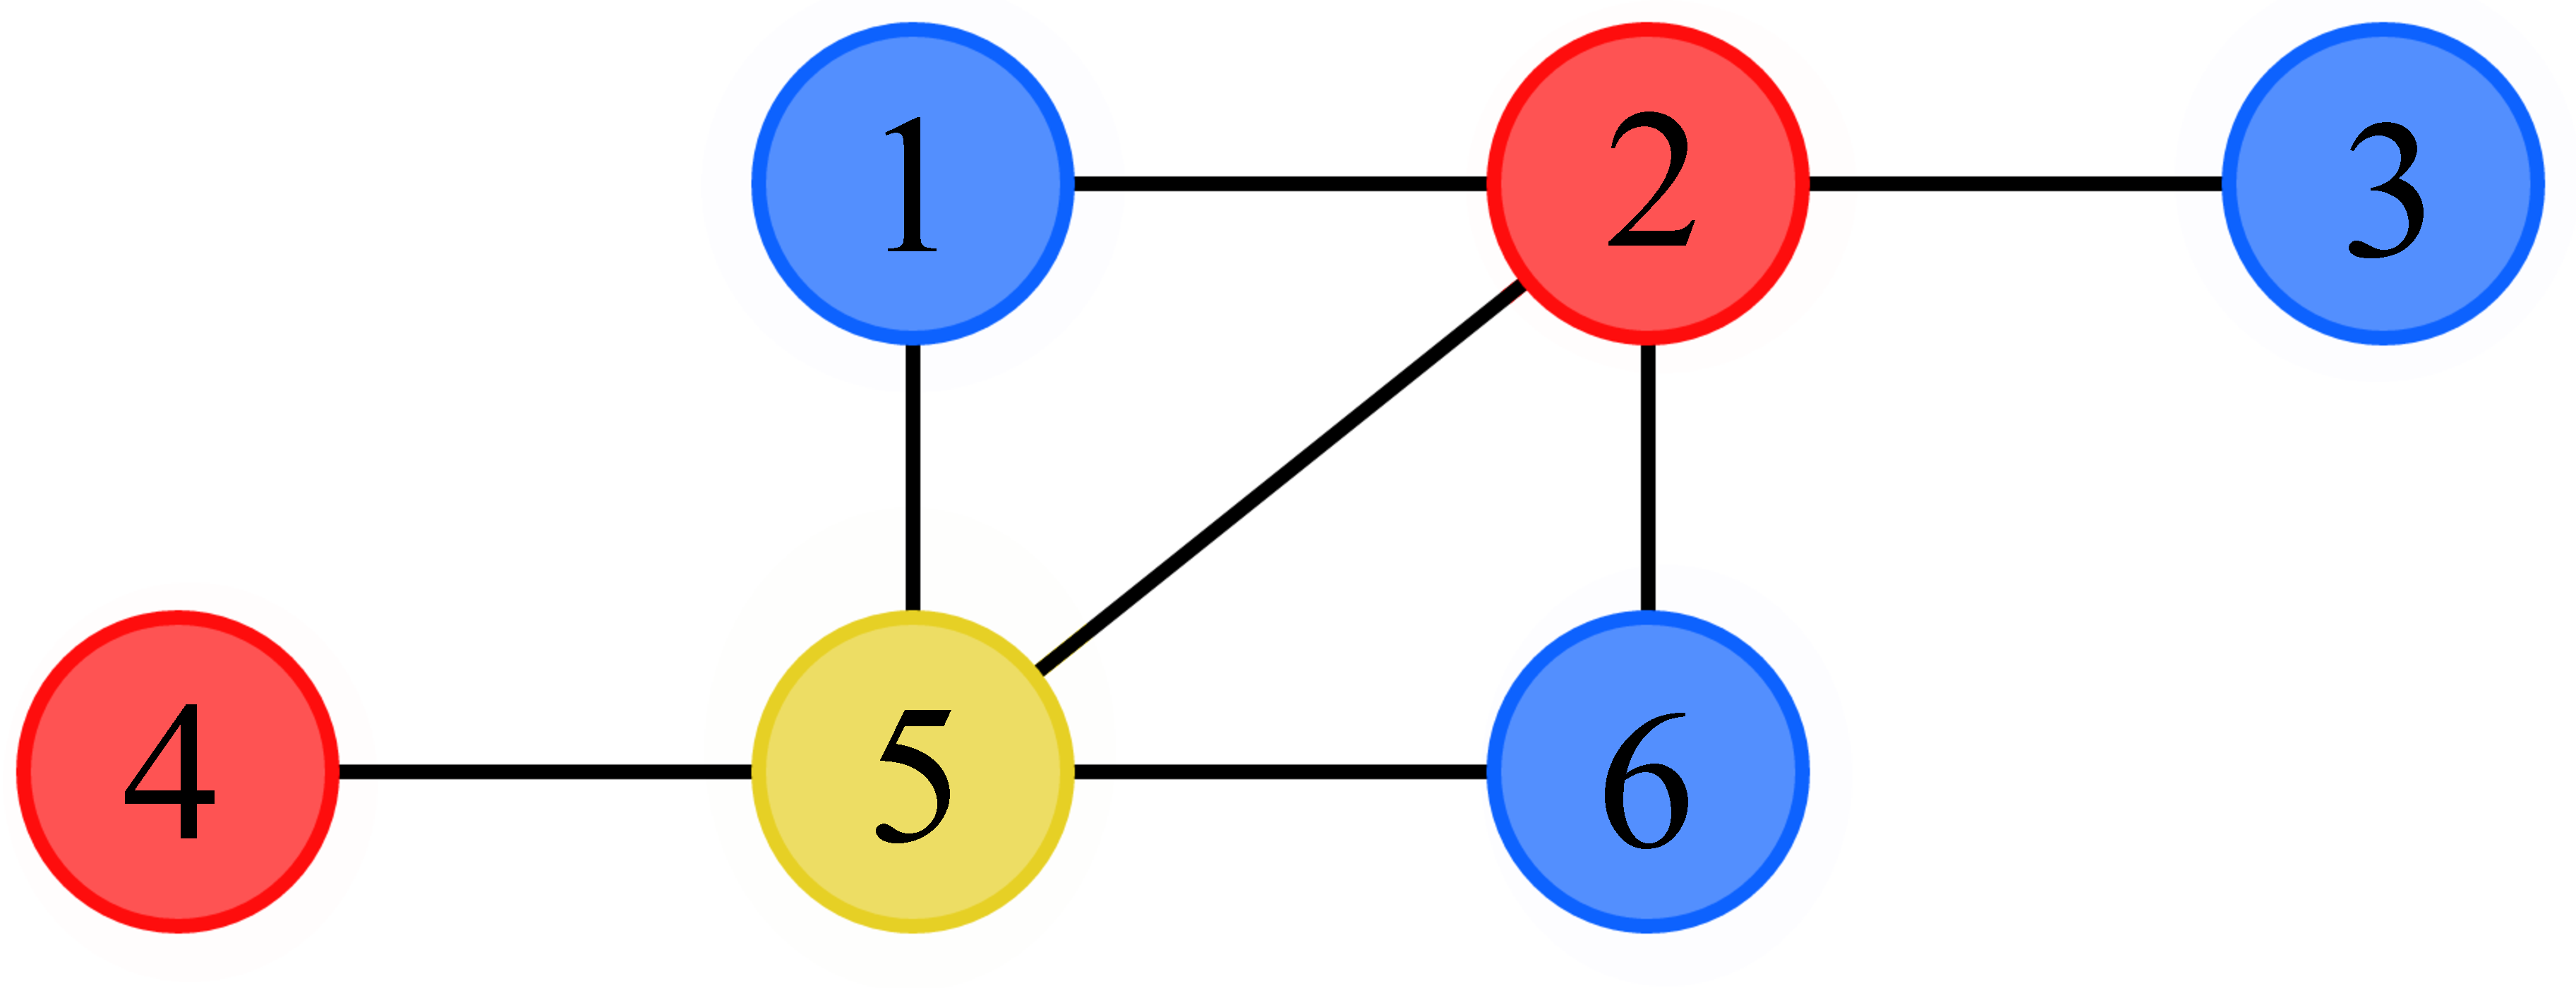
\includegraphics[width=7cm]{../figures/example-vcp.pdf}
	\caption{A minimum vertex coloring of $G_1$}\label{fig:vcp-example}
\end{figure}

\subsection{Graph Coloring}
\label{sec:coloring}
A \emph{vertex coloring} is an assignment of colors to each vertex of a graph $G$. A \emph{proper vertex coloring} assigns colors such that no two adjacent vertices share the same color. Mathematically, it can be described as a function $f : V \rightarrow S = \{1, 2, \dots, k\}$ such that $\forall u,w \in V$, if $(u,w) \in E$, then $f(u) \neq f(w)$. The \emph{chromatic number} of $G$, denoted $\chi(G)$, is the minimum number of colors needed to properly color $G$. The \emph{vertex coloring problem} (VCP), when given a simple graph $G$, is to find $\chi(G)$. \cite{bondy1976graph}

A graph $G$ is said to be \emph{k-colorable} if it can be colored using $k$ or fewer colors, i.e. $\chi(G) \leq k$. A graph having $\chi(G) = k$ is said to be a \emph{k-chromatic} graph. The \emph{k-colorability} problem asks if a graph can be colored using $k$ colors. This problem is slightly different than the VCP as it is a decision problem rather than an optimization problem. An example of a 3-colorable graph and a vertex coloring is shown in Figure \ref{fig:vcp-example}.

\begin{figure}[h]
	\centering
	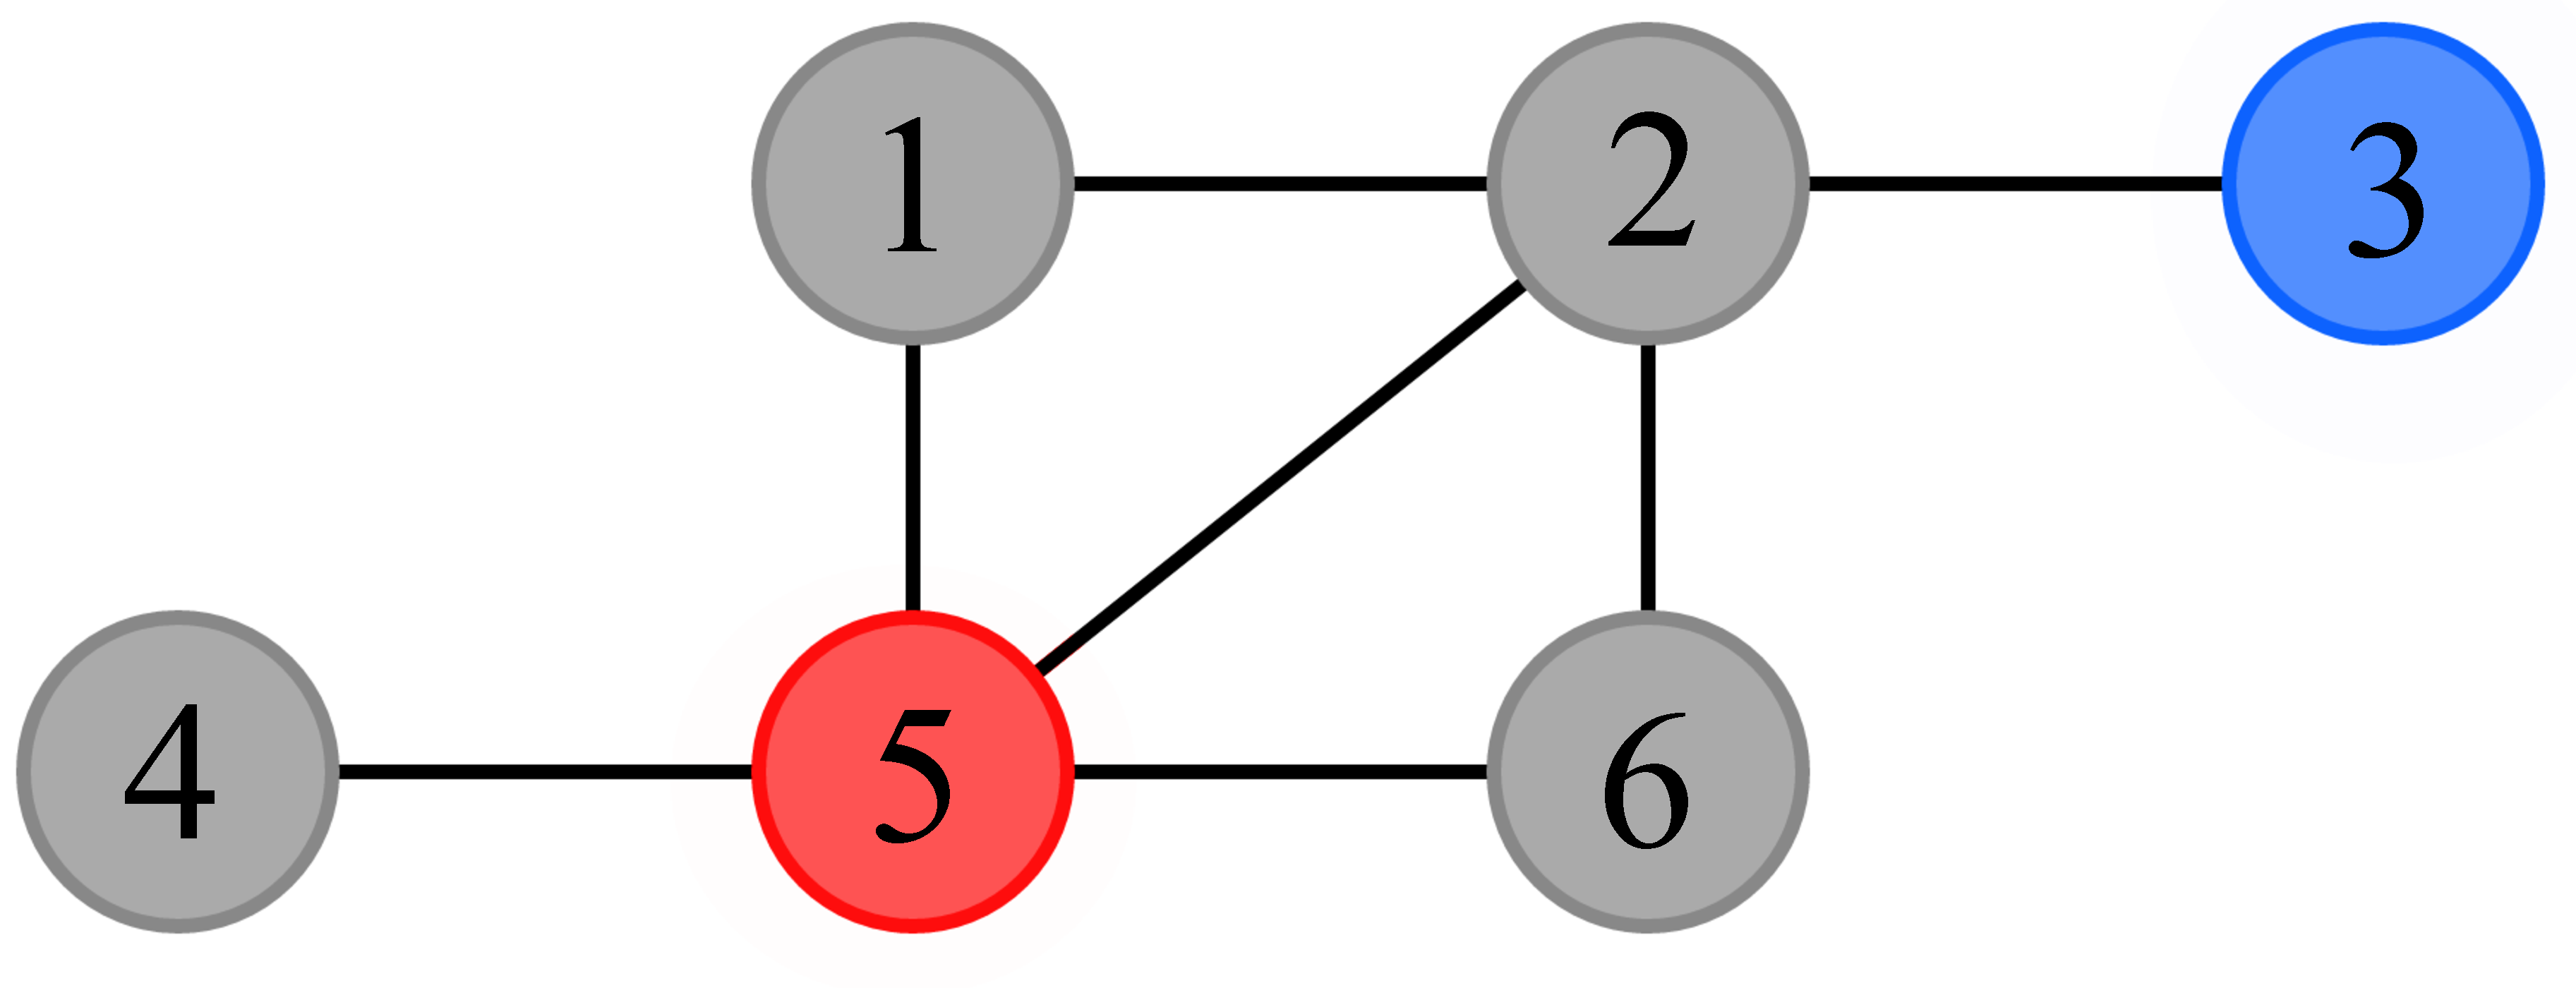
\includegraphics[width=7cm]{../figures/example-cfcp.pdf}
	\caption{A minimum conflict-free coloring of $G_1$}\label{fig:cfcp-example}
\end{figure}

A \emph{conflict-free k-coloring} of a simple graph $G$ assigns colors, $\{1, 2, \ldots, k\}$, to a subset $P \subseteq V$ of vertices such that $\forall v \in V$, there is a vertex $u \in N(v)$ where the color of $u$ is unique in the neighborhood of $v$. The set $V \setminus P$ is the uncolored vertices, if any. Generally, a \emph{conflict-free coloring} of a graph assigns colors to some of the vertices such that, for every vertex $v$, there is a unique color assigned to a vertex among $v$ and $v$'s neighbors. The vertex $u$ can be thought of the \emph{conflict-free neighbor} of $v$. The \emph{conflict-free chromatic number} of G, denoted $\chi_{CF}(G)$, is the smallest $k$ for which a conflict-free coloring exists. The \emph{conflict-free coloring problem} (CFCP) aims to find $\chi_{CF}(G)$. \cite{abel2017three}

An example of a conflict-free coloring is shown in Figure \ref{fig:cfcp-example}. All uncolored vertices are in gray. It is a valid conflict-free coloring because every vertex has a unique color within its neighborhood. For example, $N(1) = \{1: uncolored,\ 2: uncolored,\ 5: red\}$. As there are no other vertices colored red, we have verified there is a unique color in the neighborhood of vertex 1. We observe from Figures \ref{fig:vcp-example} and \ref{fig:cfcp-example}, $\chi(G_1) = 3$ and $\chi_{CF}(G_1) = 2$. It is worth noting that all proper vertex colorings are also conflict-free colorings. This is because in a proper vertex coloring, every vertex is its own conflict-free neighbor \cite{abel2017three}.

A dominating set is a subset $D$ of $V$ such that every vertex not in $D$ is adjacent to at least one vertex in $D$. The set of colored vertices in a conflict-free coloring is a dominating set \cite{abel2017three}. The domination number of $G$, denoted $\gamma(G)$, is the size of a minimum dominating set of G. An example of a dominating set is $\{3, 5\}$ of graph $G_1$ where $\gamma(G_1) = 2$. The \emph{conflict-free domination number} for some $k$, denoted $\gamma_{CF}^k(G)$, is the minimum number of vertices that have to be colored in a conflict-free k-coloring of $G$. The \emph{k-conflict-free dominating set} problem asks if a given k-coloring of a graph colors the minimum amount of vertices needed to have a conflict-free coloring that utilizes $k$ colors.

\subsection{Computational Complexity Theory}
\label{sec:complexitytheory}
A \emph{decision} problem, as mentioned earlier, is a problem that can be answered with `yes' or `no' \cite{sipser2006introduction}. A problem can be solved in polynomial time if an algorithm with input size $n$ can run in at most $n^k$ steps where $k$ is a constant that does not depend on $n$. A decision problem is said to be in the class \emph{P} if in the worst case, it can be solved with an algorithm that runs in polynomial time.

Given a decision problem and a proposed solution, it can be possible to verify the answer quickly. If a decision problem can be verified in polynomial time but not necessarily solved in polynomial time, it is said to be in the class \emph{NP}. Take note that this does not exclude problems in class P; P is a subset of NP.

There are certain problems, called NP-hard, that can be proven to be as hard as every problem in NP. If problem $Y$ can be transformed into problem $X$ by a polynomial-time algorithm, it is said that $Y$ can be polynomially reduced to $X$. A problem is NP-hard if it every problem in NP can be polynomially reduced to it. This means that if an NP-hard problem can be solved with a polynomial-time algorithm, then any problem in NP could be solved in polynomial time. A decision problem is said to be \emph{NP-complete} when it is both in NP and NP-hard.

The k-colorability problem as well as the conflict-free k-colorability problem are NP-complete. This can be proven by using a reduction from a known NP-complete problem \cite{garey2002computers}. If we find a known hard problem $Y$, we can prove that another problem $X$ is hard by a reduction from $Y$ to $X$. The VCP and the CFCP have both been shown to be NP-hard \cite{abel2017three,moret1998theory}. The k-colorability problem is proven to be NP-complete with a reduction from 3-SAT, another well-known NP-complete problem \cite{sharma2012new}. The conflict-free k-colorability problem is shown to be NP-complete by a reduction from k-colorability \cite{abel2017three}.

It is often desirable and necessary to use approximation algorithms, called heuristics, to solve complex problems like the VCP and the CFCP. In our case, heuristics are polynomial-time algorithms that give good, but not optimal, solutions to our optimization problems. A polynomial-time approximation scheme (PTAS) is any polynomial-time approximation algorithm that takes an instance of an optimization problem and a parameter $\epsilon > 0$ and produces a solution that is within a factor $(1 + \epsilon)$ (for minimization problems) of being optimal.

\vspace{-0.2cm}

\section{Applications}
Before digging into methods for solving the CFCP, it is important to understand what motivated the recent studies into conflict-free coloring.

\subsection{Wireless Networks}
The main application for conflict-free coloring surrounds wireless networks. Cellular networks, radio, television broadcasting, and satellite communication utilize some form of wireless networks. For each of these systems, a frequency assignment problem arises with specific characteristics.

For example, imagine a cellular network. Cellular networks are heterogeneous networks with two different types of nodes. They have \emph{base-stations} (servers) and \emph{clients}. Base stations are all interconnected through an external backbone network. Clients can only be connected to base stations and connect via radio links. Base stations are each assigned a fixed frequency. Clients, however, are constantly searching frequencies for base-stations with strong reception.

The main problem when initially setting up these networks comes into play when assigning frequencies. Imagine two base-stations near each other having the same frequency. If a client is in reception range of both base-stations, then mutual interference occurs and the radio link is too noisy to be used for proper communication. The goal is to assign frequencies to base stations such that every client is served by some base-station and to minimize the number of frequencies used.

\begin{figure}[h]
	\centering
	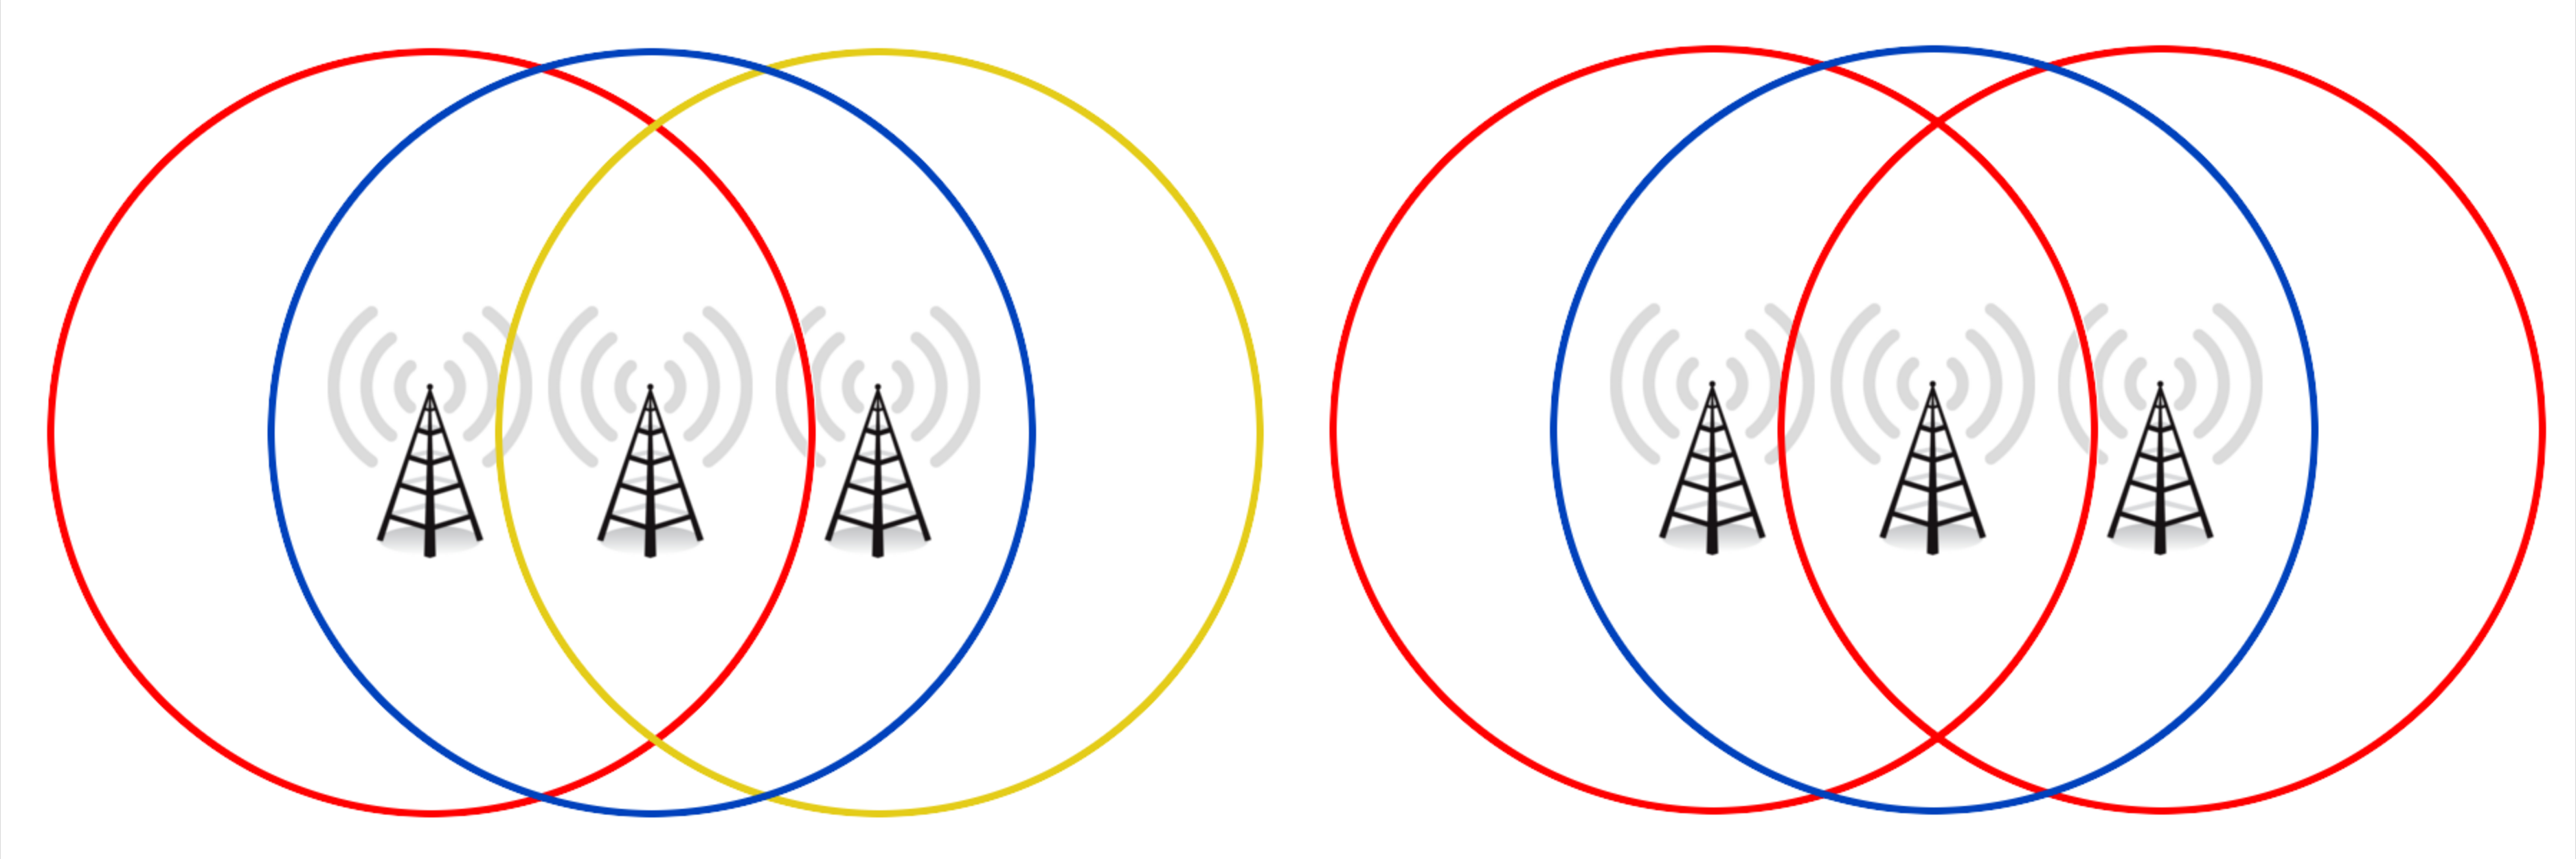
\includegraphics[width=8cm,trim=4 4 4 4,clip]{../figures/towers.pdf}
	\caption{Cellular tower VCP and CFCP example}\label{fig:towers}
\end{figure}

\vspace{-0.1cm}

This problem was initially modeled as a vertex coloring problem, where the vertices are the base-stations and the edges are the pairs of base-stations that overlap in their reception range. This model is too wasteful and restrictive. Imagine a situation where a client is within the reception range of 3 base-stations. The VCP model would require 3 colors, one for each base station. If we assign one base-station a color (say blue) and the other 2 a \emph{different} color (say red), then we only utilize two colors and the client utilizes the blue base-station and has no mutual interference. This model is shown in Figure \ref{fig:towers}. This is exactly what a conflict-free coloring does. \cite{smorodinsky2013conflict}

\subsection{RFID Networks}
Radio frequency identification (RFID) networks are similar to wireless networks. An object, such as a credit card with an RFID chip, has a specific tag attached to it. A reader, such as a credit card scanner, can sense the presence of this object and read an ID that is assigned to the tag of the object. RFID is used for tracking progress of automobiles through a production assembly line, timing marathons and races, security access control to parking garages and buildings, and much more.

Multiple RFID readers are often set up in a given location to improve coverage of the overall area. There can also be multiple RFID readers set up that each do a different action after reading a tagged object. Unlike cellular towers, a reader can only be reading (i.e. connected to) a single tag at a time. Two readers trying to access a tagged object at the same time can cause mutual interference. The goal is to schedule for each reader a time slot for when the reader will be active.

Imagine we have a set of readers, $R$. Suppose they all are assigned the same frequency. We would like to schedule each reader $r \in R$ a time slot $t(r)$ where the reader $r$ will be active. We have a set of tags $P$ (i.e. product RFID chips). We can say that $P$ is read by our schedule if for every tag $p \in P$, there is at least one reader $r \in R$ and a time $t$ such that $p$ is read by $r$ at time $t$. We want to minimize the total time slots used by the schedule. This can be accomplished by modeling the situation as a conflict-free coloring problem. Again, we aim to find the minimum number of colors needed. \cite{cheilaris2014strong, smorodinsky2013conflict}

\section{CF Coloring of General Graphs}
\label{sec:general-coloring}
For this section, we will consider the NP-complete problem of conflict-free k-colorability. Given a graph $G$ and an integer $k$, determine if graph $G$ can be colored using $k$ or fewer colors. Although all graphs can be conflict-free colored, a given graph $G$ may not be able to be colored with $k$ colors.

As shown with graph $G_1$ in section \ref{sec:background}, even though all proper vertex colorings are also conflict-free colorings, fewer colors can usually be used. This leads us to use heuristics that differ from the vertex coloring problem. Abel et al. \cite{abel2017three} present an efficient heuristic to color certain general graphs with $k$ colors in a conflict-free manner. They call this heuristic \emph{iterated elimination of distance-3-sets}.

\subsection{Guaranteeing CF k-Colorability}
It is wasteful to spend time coloring a graph that cannot be conflict-free colored. This leads Abel et al. to provide sufficient criterion to guarantee the conflict-free k-colorability of a certain graphs. To introduce this criterion, we need to introduce a few specific graphs. A complete graph is a simple, undirected graph where every pair of distinct vertices is connected by an edge. A complete graph on $n$ vertices is denoted as $K_n$. The graph $K_n^{-3}$ is the graph obtained by removing any three edges forming one single triangle, i.e. $K_3$.

A graph $H$ is called a \emph{minor} of a graph $G$ if $H$ can be formed by deleting edges and/or contracting edges (combining the vertices of an edge) from $G$. \cite{abel2017three,bondy1976graph}

\begin{theorem} \label{thm:criterion}
Let $G$ be a graph and $k \geq 1$. If $G$ has neither $K_{k+2}$ nor $K_{k+3}^{-3}$ as a minor, $G$ has a conflict-free coloring that can be found in polynomial time using iterated elimination of distance-3-sets.
\end{theorem}

Abel et al. give a criterion that guarantees k-colorability which is stated in Theorem \ref{thm:criterion}. In the proof of this theorem, found in \cite{abel2017three}, the authors prove that their heuristic, given in section \ref{sec:iterated}, will always generate a k-colorable graph when the specified criterion is met.

\subsection{Setting Up Example CF Coloring}
Before demonstrating Algorithm \ref{alg:elimination}, we will demonstrate how to check if a graph, say $G_2$ in Figure \ref{fig:criterion}, meets the given criterion.

\begin{figure}[h]
	\centering
	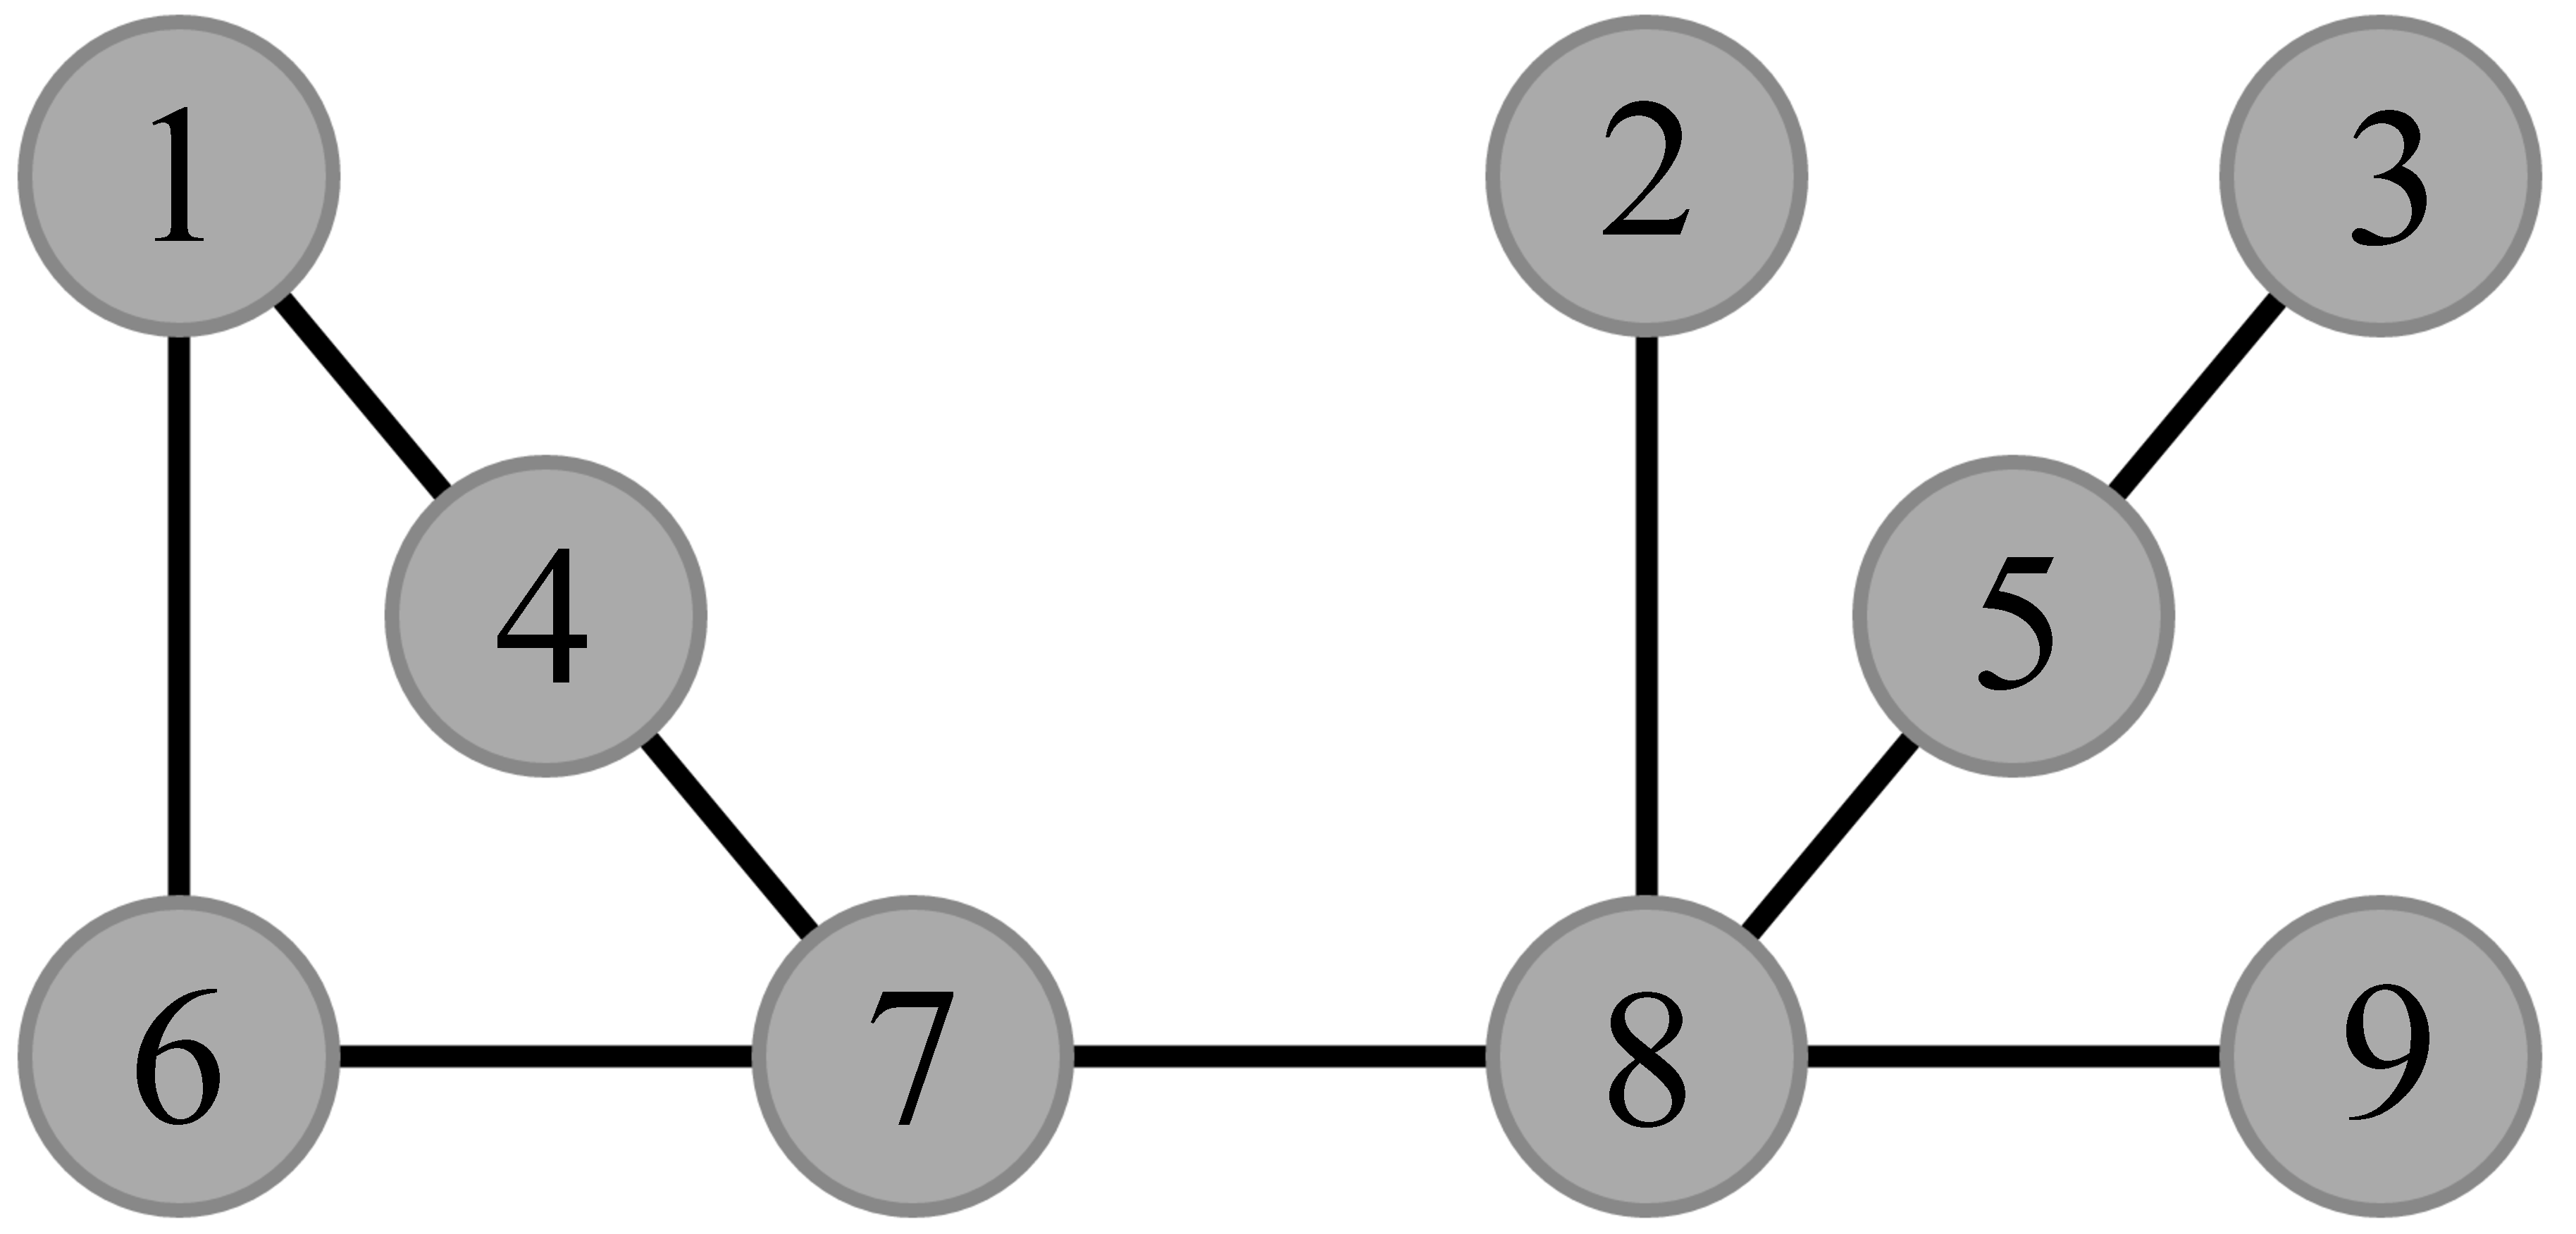
\includegraphics[width=6cm]{../figures/criterion.pdf}
	\caption{A simple graph $G_2$}\label{fig:criterion}
\end{figure}

We will be focusing on the simplest example, $k = 1$. Graph $G_2$ is a simple graph with 6 vertices. For $k = 1$, this means our graph cannot contain $K_{3}$ or $K_{4}^{-3}$ as a minor. These graphs are shown in Figure \ref{fig:bad-criterion}.

\begin{figure}[h]
	\centering
	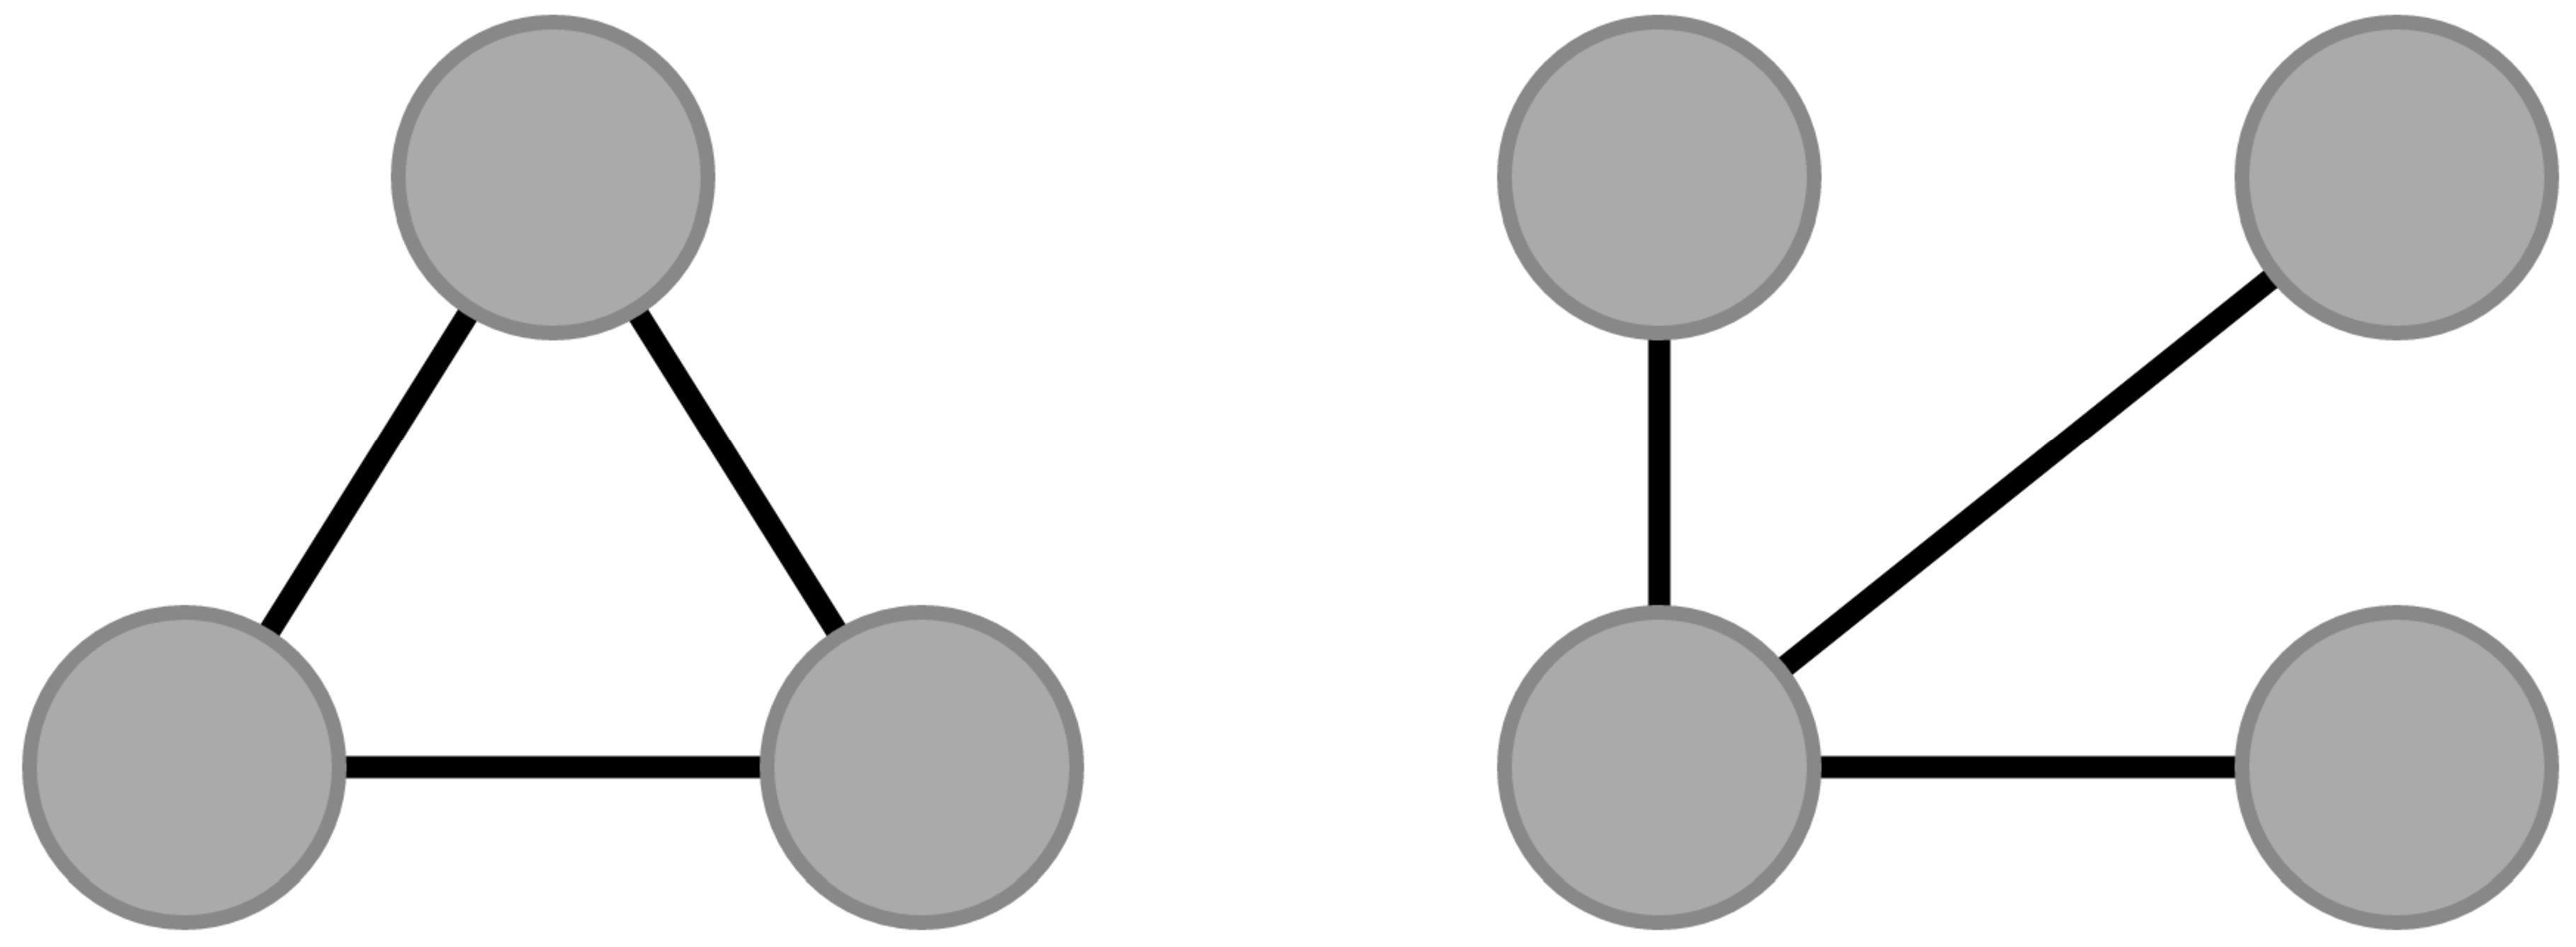
\includegraphics[width=6cm]{../figures/bad-criterion.pdf}
	\caption{Graphs $K_{3}$ and $K_{4}^{-3}$, respectively}\label{fig:bad-criterion}
\end{figure}

We can see that $G_2$ has both of these as minors. The transformation needed to see the minors is shown in Figure \ref{fig:criterion-minor}. By contracting the dotted edges, vertices 1 and 4 would combine as well as vertices 3 and 5. We would have both $K_{3}$ and $K_{4}^{-3}$. This graph does not fit our criterion; it even breaks both properties as it has both $K_{k+2}$ and $K_{k+4}^{-3}$ as a minor. Thus, this graph cannot be conflict-free colored with one color.


\begin{figure}[h]
	\centering
	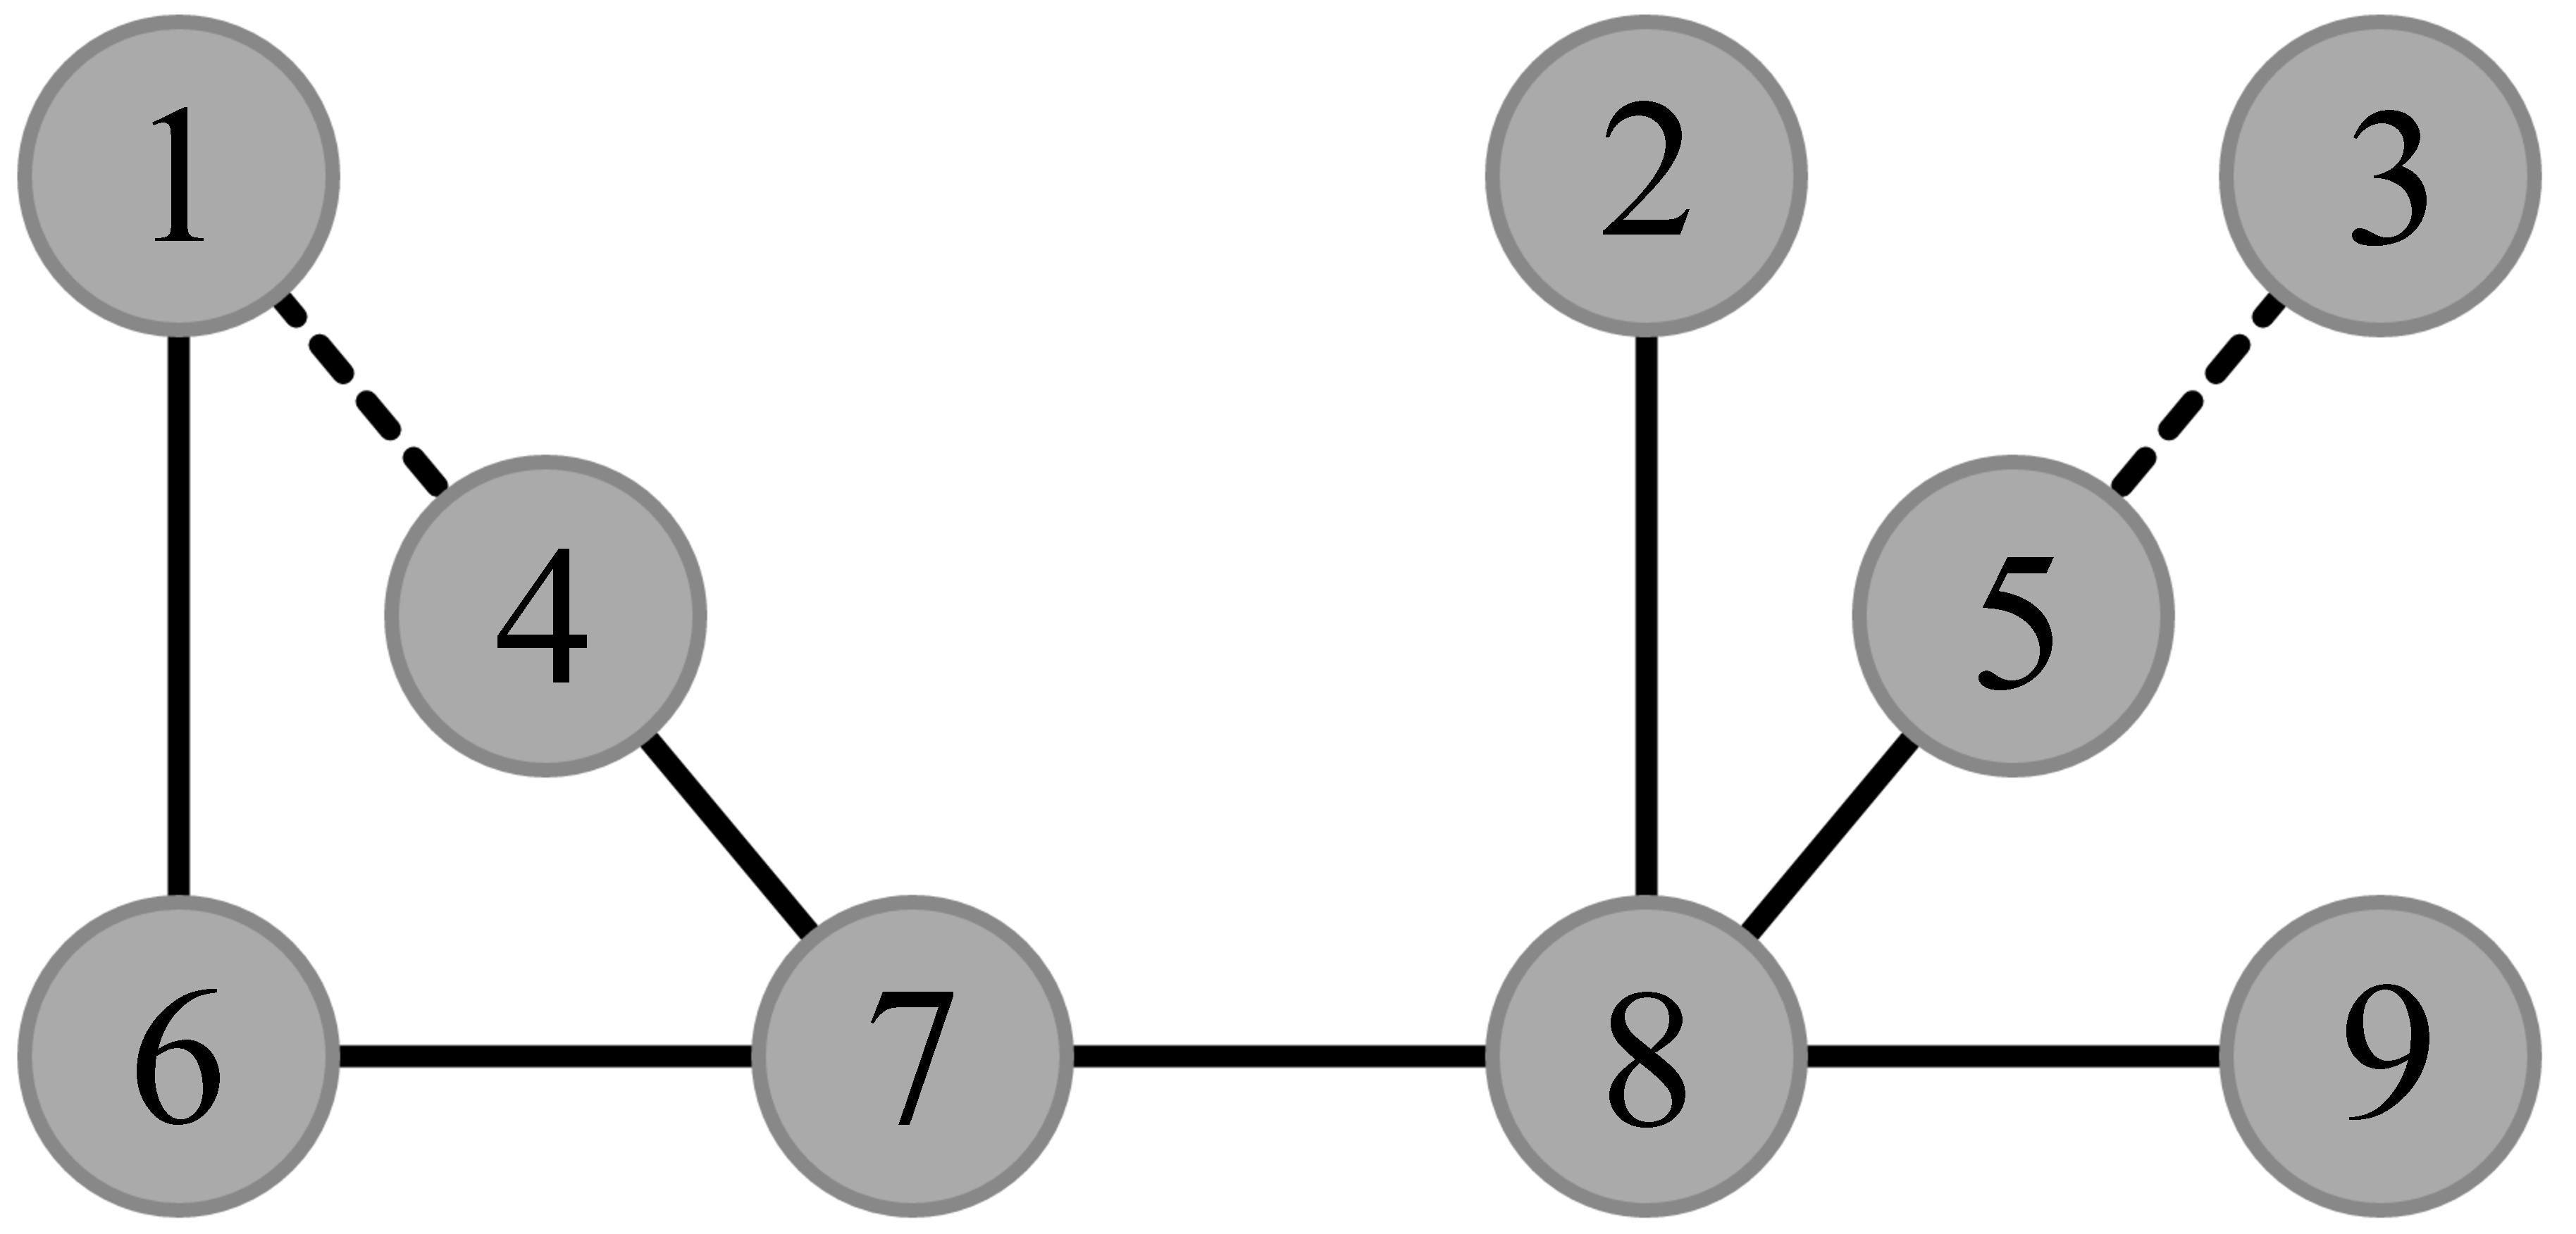
\includegraphics[width=6cm]{../figures/criterion-minor.pdf}
	\caption{How to transform $G_2$ to see the minors}\label{fig:criterion-minor}
\end{figure}

\vspace{-0.1cm}

\subsection{Iterated Elimination of Distance-3-Sets}
\label{sec:iterated}
The iterated elimination of distance-3-sets algorithm, defined in \cite{abel2017three} and shown in Algorithm \ref{alg:elimination}, is a polynomial-time heuristic for generating a conflict-free k-coloring of general graphs that satisfy the criterion given in Theorem \ref{thm:criterion}. If the criterion is not met, the heuristic will produce a conflict-free coloring of more than $k$ colors.

\begin{algorithm}
\caption{Iterated elimination of distance-3-sets} \label{alg:elimination}
\begin{algorithmic}[1]
\Input A simple, undirected graph $G$
\State $i \gets 1$
\State Remove all isolated paths from $G$
\While{$G$ is not empty}
	\State $D \gets \emptyset$
	\ForAll{components of $G$}
		\State Pick any vertex $v$
		\State $D \gets D \cup \{ v \}$
		\While{$\exists u$ at distance $\geq 3$ $\forall v \in D$}
			\State Pick $u$ at distance 3 from some vertex in $D$
			\State $D \gets D \cup \{ w \}$
		\EndWhile
		\ForAll{$u \in D$}
			\State Color $u$ with color $i$
		\EndFor
		\State $i \gets i + 1$
		\ForAll{$u \in D$}
			\State Remove $N(u)$ from $G$
		\EndFor
		\State Remove all isolated paths from G
	\EndFor
\EndWhile
\State Color all removed isolated paths using color $i$
\end{algorithmic}
\end{algorithm}

To illustrate this algorithm and show it produces a valid conflict-free coloring, we'll use graph $G_3$ shown in Figure \ref{fig:algorithm1}. The algorithm starts by setting a variable $i$, the current color, to a (color) 1. We then remove all isolated paths from the input graph. There are currently no isolated paths in $G_3$, so we do not remove anything.

Since $G_3$ is not empty, we enter the first $while$ loop and set a variable $D$ to the empty set. $G_3$ has only one component (the whole graph) so we will only iterate through the \emph{for all} on line 5 once. Pick any vertex from $G_3$, say vertex 8. We then add 8 to set $D$ and thus $D \gets \{8\}$. Now, while there exists a vertex with a distance of at least 3 from all vertices in $D$, we must pick a vertex of exactly distance 3 and add it to $D$. For example, vertex 2 has distance 3 from vertex 8. Now, we add vertex 2 to $D$ and now $D \gets \{2, 8\}$.

\begin{figure}[h]
	\centering
	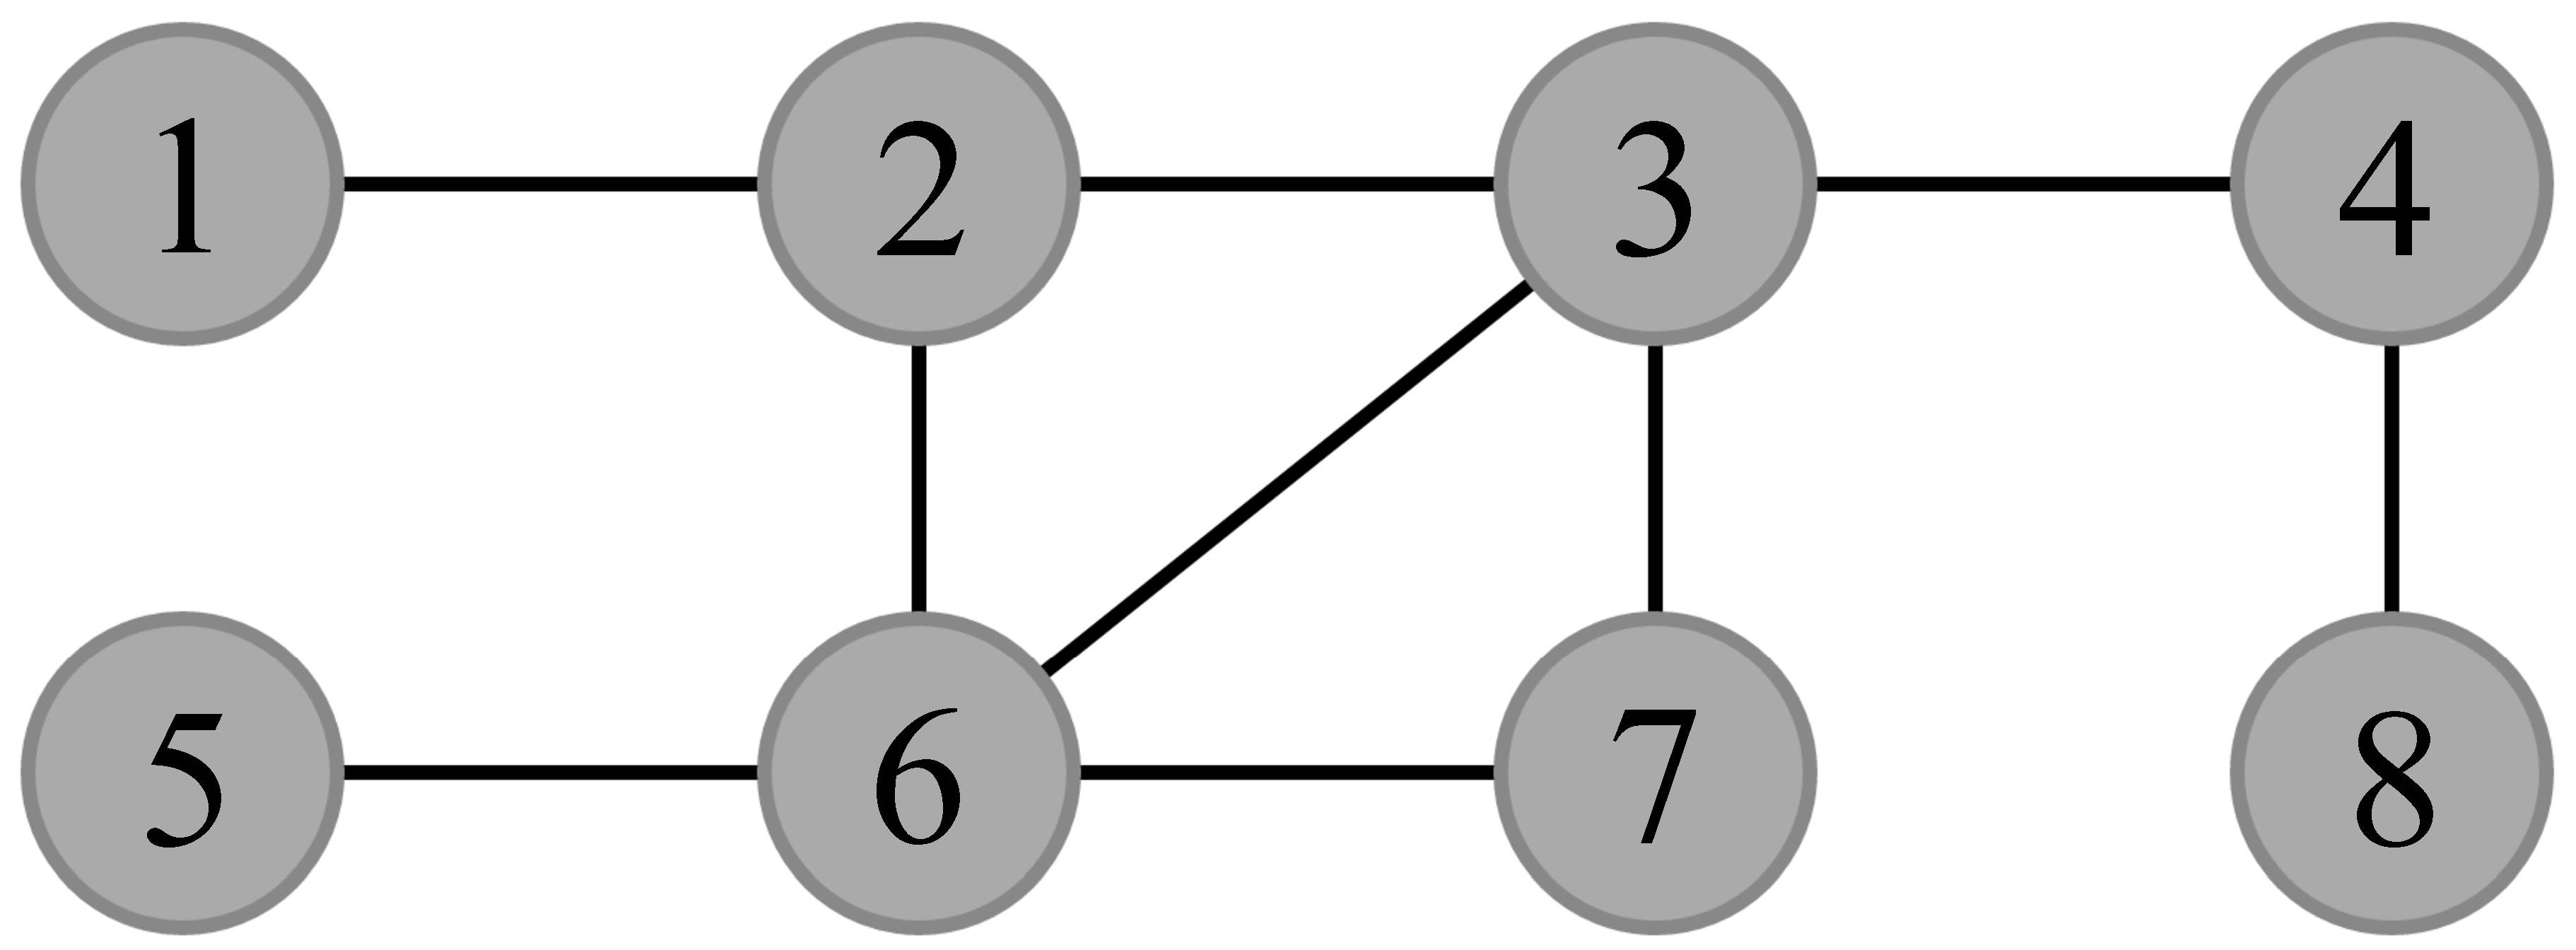
\includegraphics[width=6cm]{../figures/algorithm1.pdf}
	\caption{Graph $G_3$ to illustrate Algorithm \ref{alg:elimination}}\label{fig:algorithm1}
\end{figure}

There are no more vertices of at least distance 3 from all vertices in $D$, so we move on to line 11. We color all vertices in $D$, $\{2,8\}$, with color $i$ which is known as color 1 (say red). This coloring is shown in Figure \ref{fig:algorithm1-step1}. We increase $i$ by one leading to $i \gets 2$.

\begin{figure}[h]
	\centering
	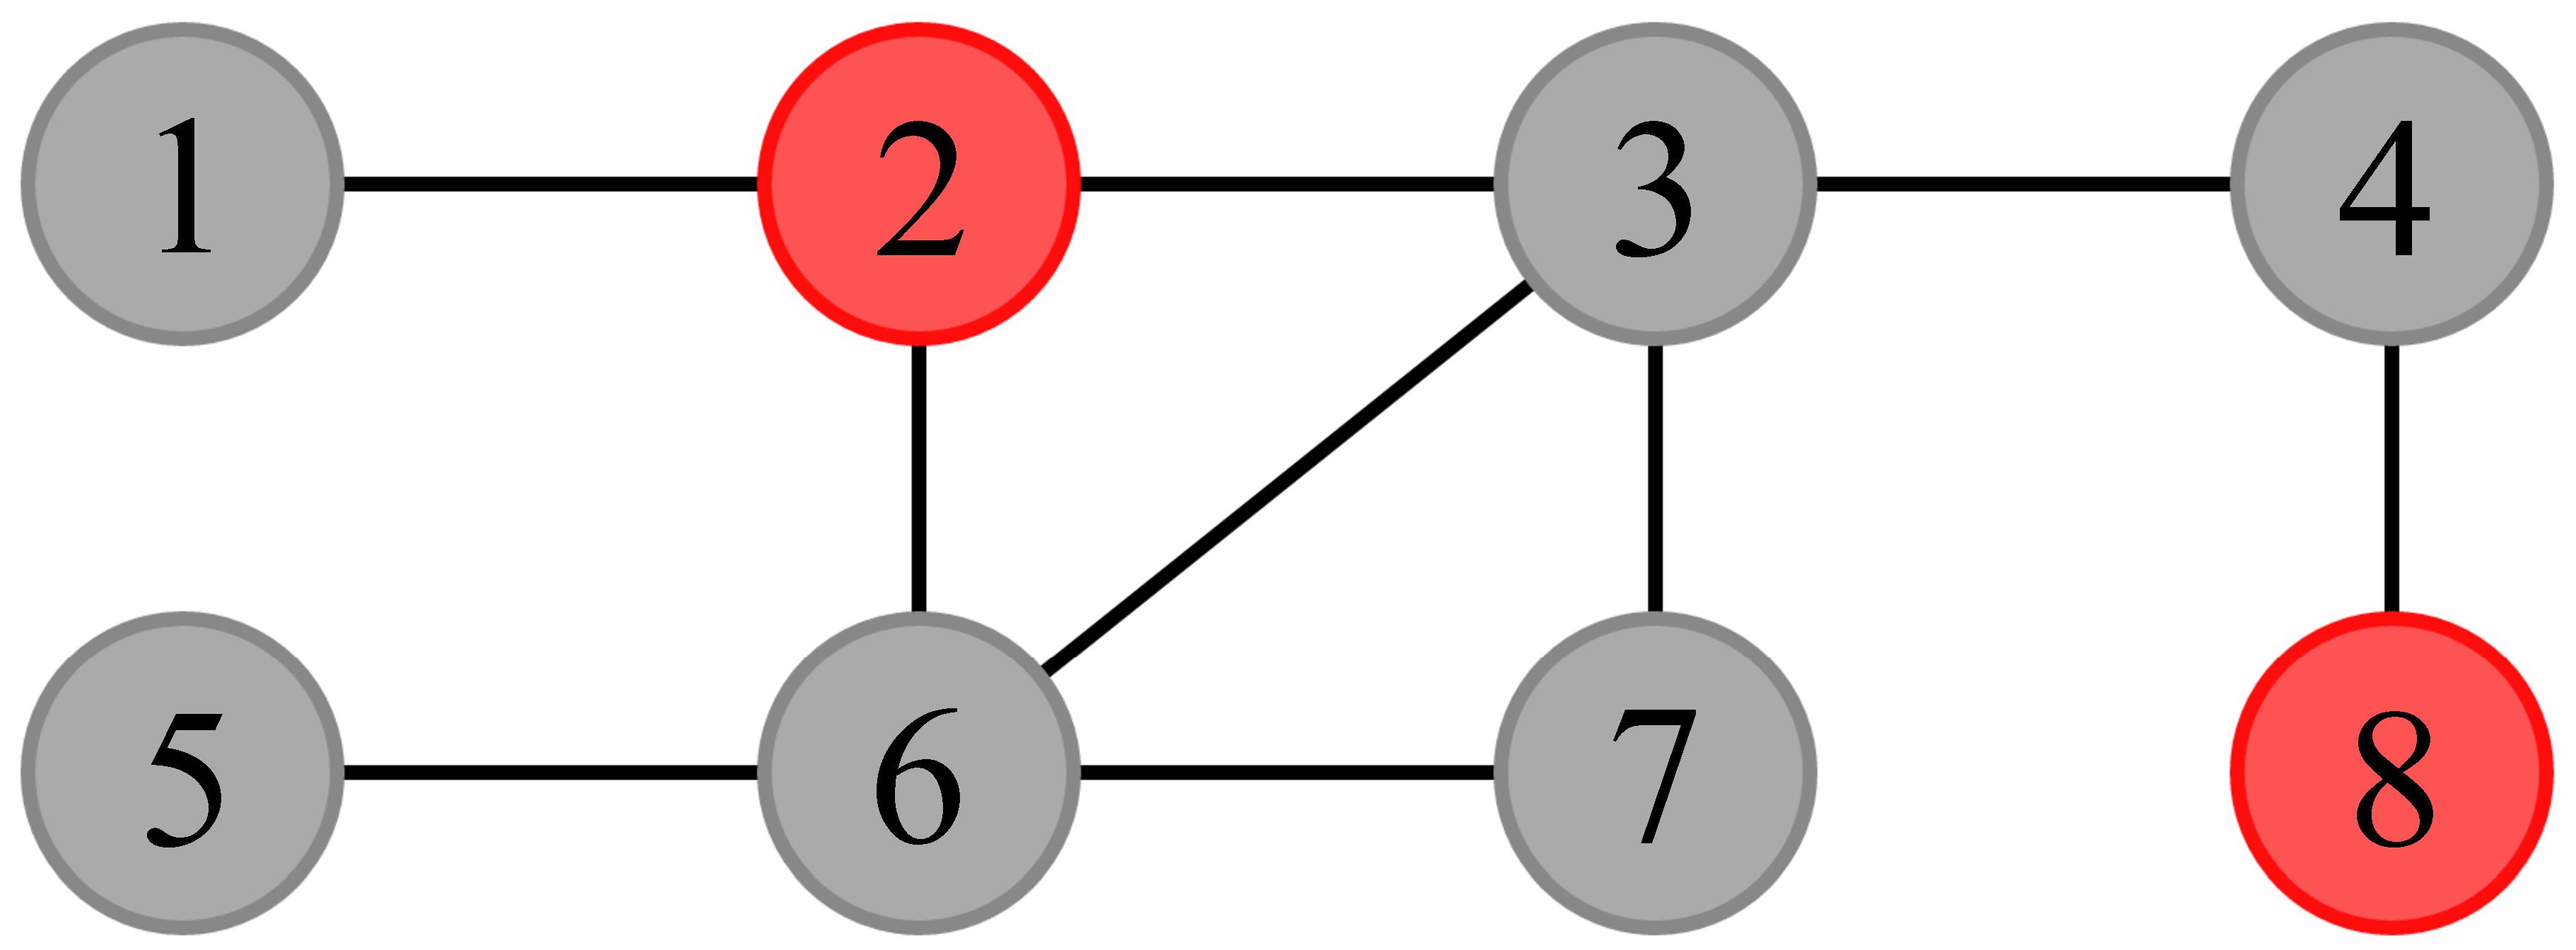
\includegraphics[width=6cm]{../figures/algorithm1-step1.pdf}
	\caption{Graph $G_3$ after lines 1-13}\label{fig:algorithm1-step1}
\end{figure}

Next, for every vertex in $D$, we must remove their closed neighborhood from the graph. The neighborhood of vertex 2 consists of $\{1,2,3,6\}$ and the neighborhood of vertex 8 consists of $\{4,8\}$. By removing these vertices and any edges containing these vertices, we are left with vertices $\{5, 7\}$.~This is shown in Figure \ref{fig:algorithm1-step2}.

\begin{figure}[h]
	\centering
	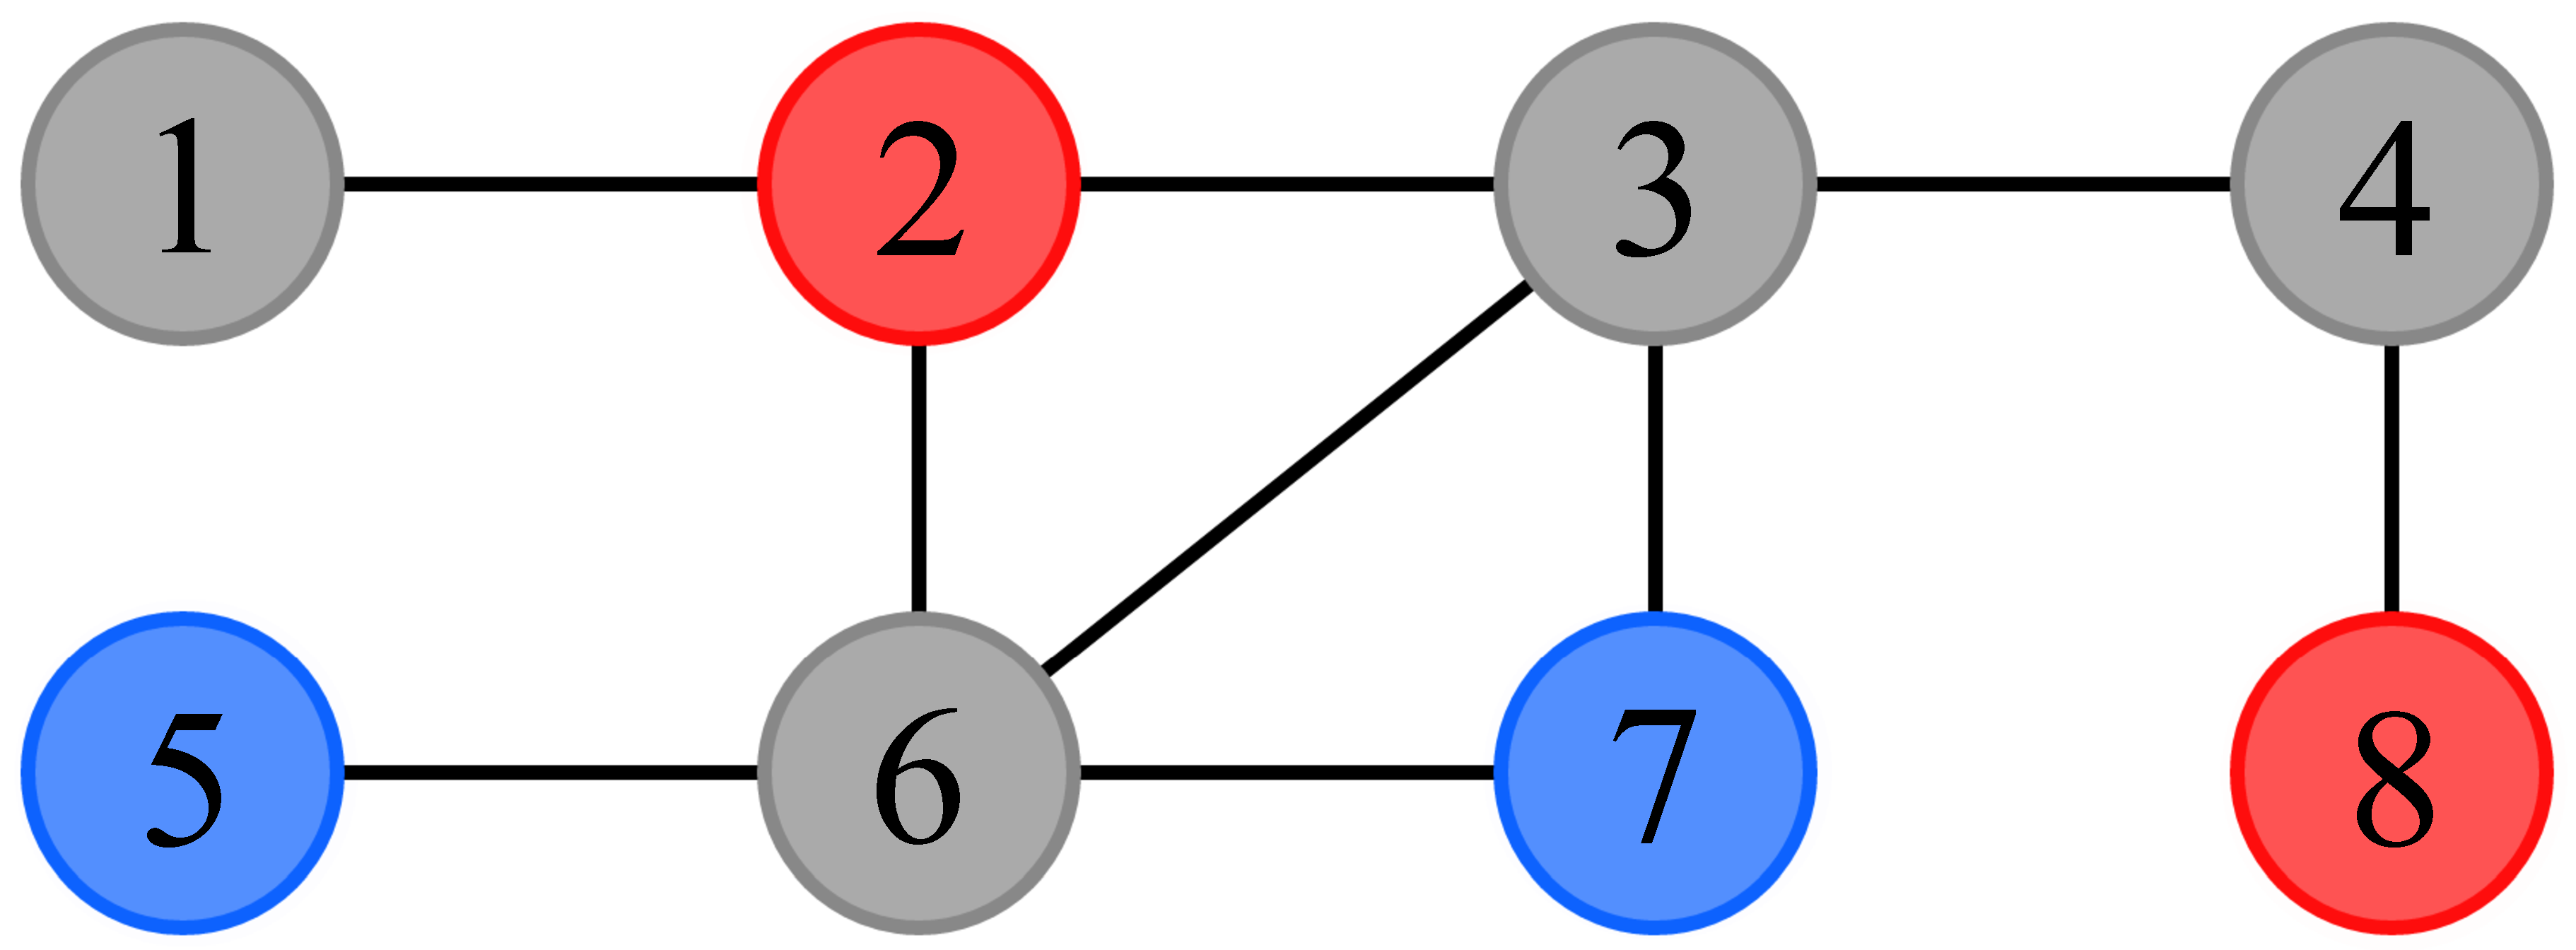
\includegraphics[width=5cm]{../figures/algorithm1-step2.pdf}
	\caption{Graph $G_3$ after lines 14-15}\label{fig:algorithm1-step2}
\end{figure}


The last step of the algorithm is to remove all isolated paths from $G$. Since we are left with only two isolated vertices, which are trivially isolated paths, we have 2 isolated paths. We remove these isolated paths from $G$ and are left with an empty graph. Since the graph is empty, we exit the outer $while$ loop and execute line 17. We color all removed isolated paths using color $i$, which is color 2 (say blue). Since we had 2 isolated paths, which are really just two vertices 5 and 7, we color each vertex with color 2.

\begin{figure}[h]
	\centering
	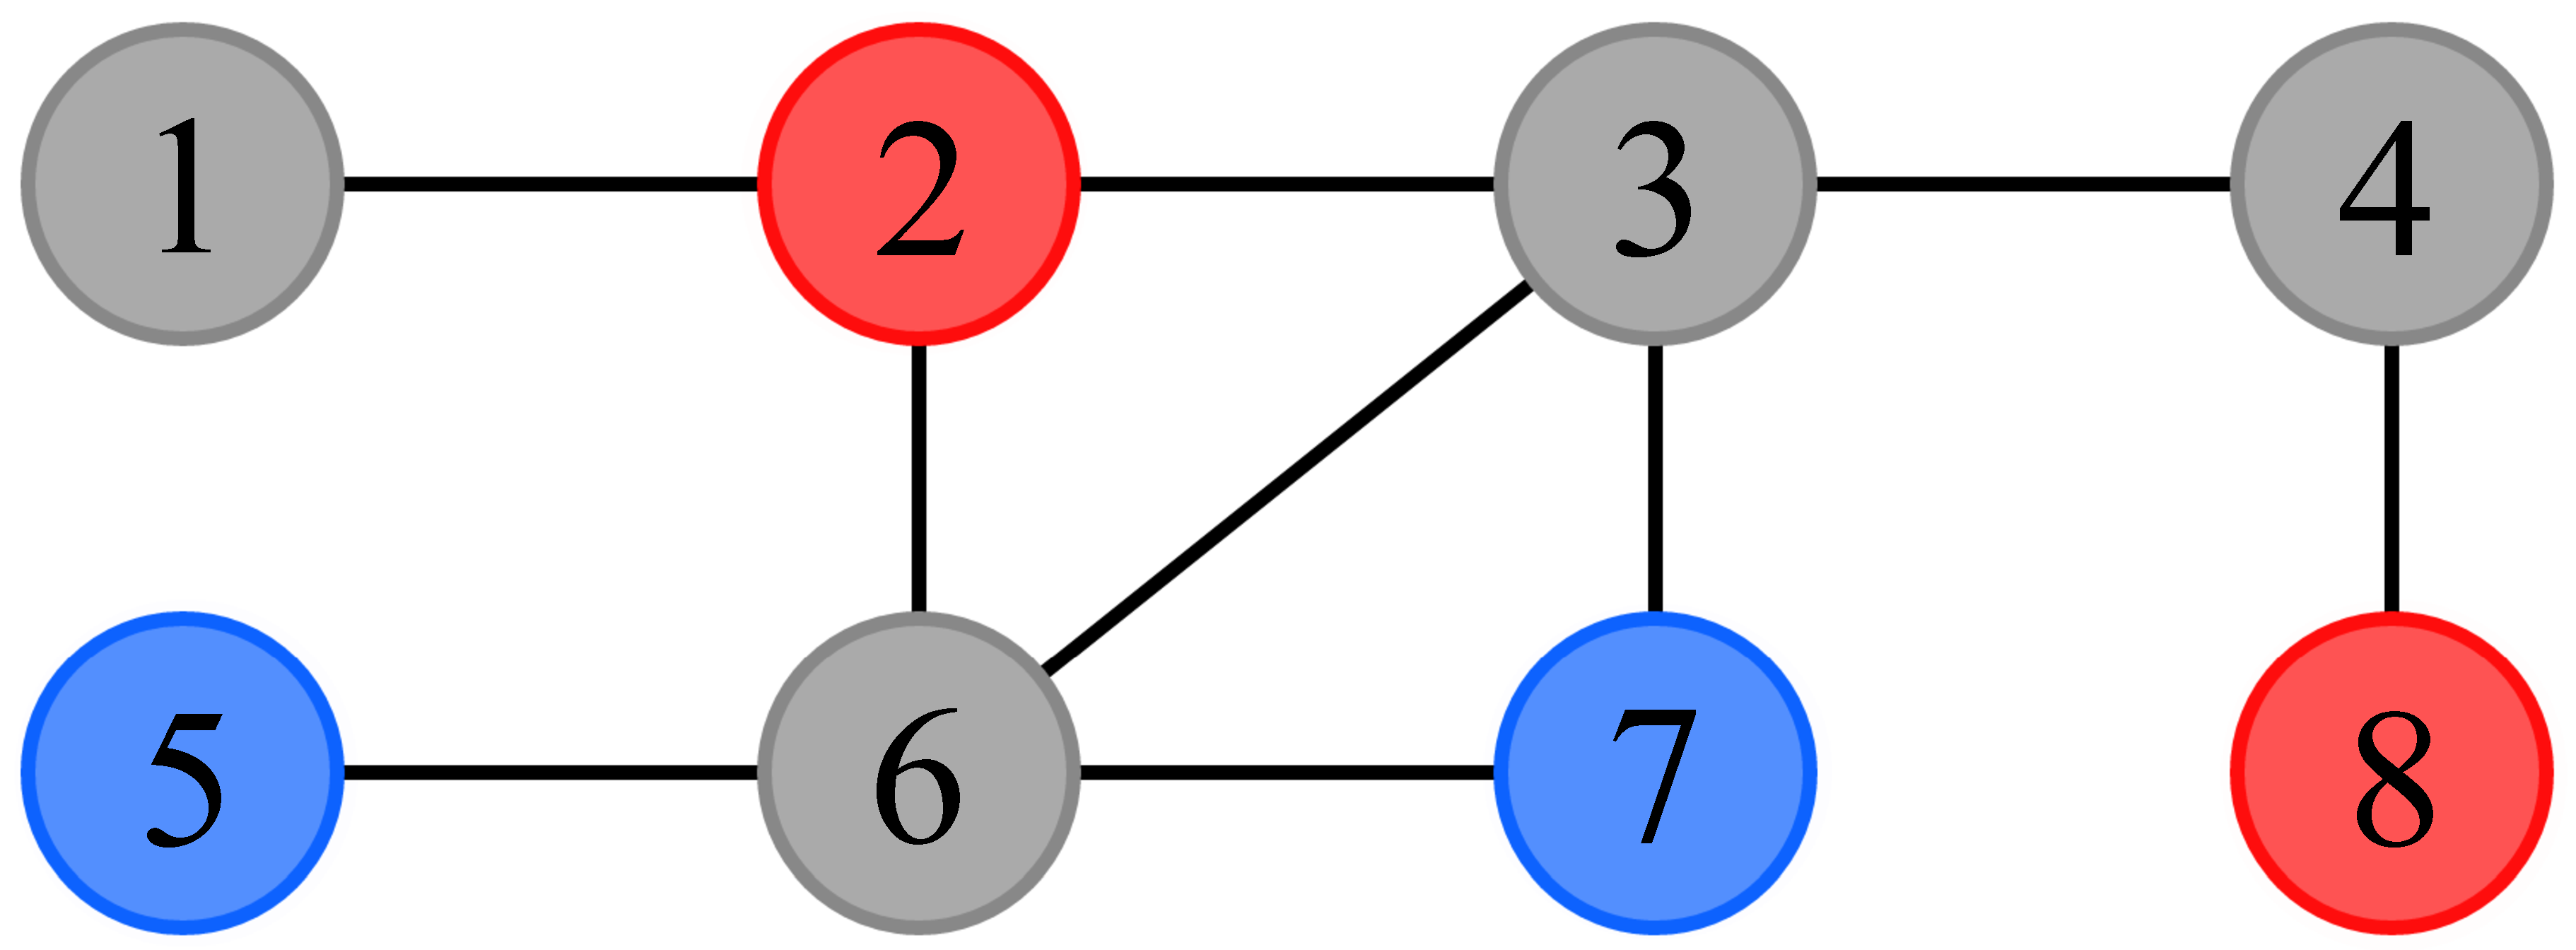
\includegraphics[width=6cm]{../figures/algorithm1-step3.pdf}
	\caption{Coloring of $G_3$ based on algorithm}\label{fig:algorithm1-step3}
\end{figure}

It was easy to color our removed isolated paths as they consisted solely of a vertex. In a more complex example, an isolated path is colored by coloring the middle vertex of every three vertices \cite{abel2017three}. This graph is not 1-colorable as it includes $K_3$ as a minor. As we have shown that this graph is 2-colorable and Theorem \ref{thm:criterion} shows it is not 1-colorable, we can conclude that $\chi_{CF}(G_3) = 2$.

It is wise to note that this algorithm does not necessarily minimize the number of colored vertices. It can be beneficial to minimize the number of colored vertices (less cost) in certain applications such as building wireless networks. The conflict-free domination number for $k=2$ of $G_3$, $\gamma_{CF}^2(G_3)$, is three even though we have four colored vertices in our example. This can be seen by coloring vertices $\{2, 8\}$ with one color and vertex 6 with another.

\section{CF Coloring of Planar Graphs}
\label{sec:planar-coloring}
Conflict-free coloring has some interesting properties when we limit the input graph to be a planar graph. Recall that a graph is planar if it can be drawn on the plane in such a way that its edges intersect only at their endpoints.

\subsection{Bounds for Planar Graphs}
\label{sec:bounds}
Recall the map of the USA example given in the introduction. This is an example of a planar graph and illustrates a famous theorem associated with it. We present this theorem, called the four color theorem, in Theorem \ref{thm:four}. The most widely-accepted proof, which utilizes a computer to brute force every possible case, can be found in \cite{robertson1997four}.

\begin{theorem} \label{thm:four}
Every loopless planar graph admits a vertex coloring with at most four distinct colors.
\end{theorem}

Due to Theorem \ref{thm:four}, we immediately know that every planar graph is conflict-free 4-colorable. This raises the question of whether there are planar graphs that require four colors or if fewer colors could suffice for all planar graphs. This leads us to the conflict-free variation of this theorem. We present this in Theorem \ref{thm:four-cf}. It is given and proven in \cite{abel2017three}.

\begin{figure}[h]
	\centering
	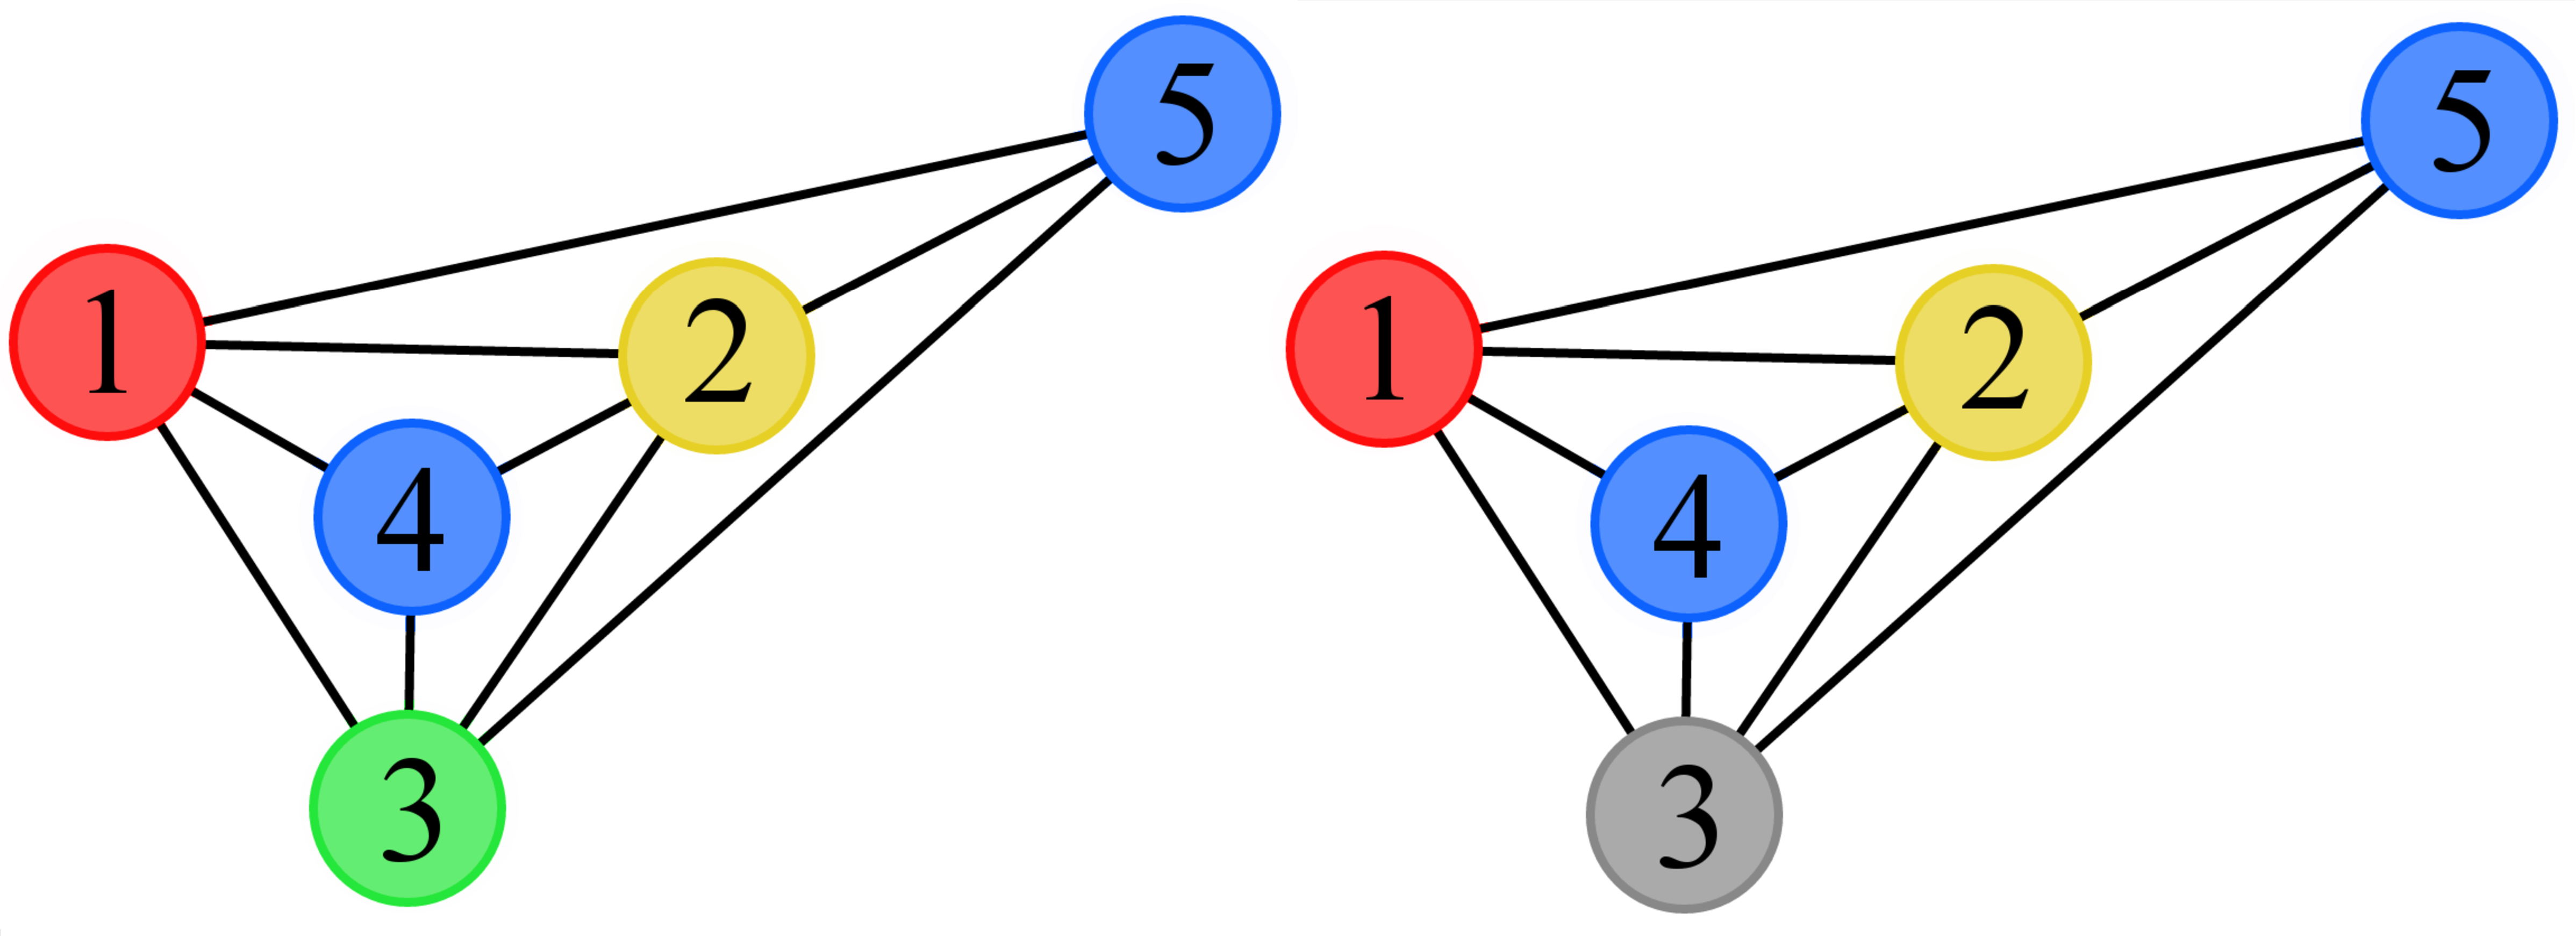
\includegraphics[width=8cm,trim=4 4 4 4,clip]{../figures/four.pdf}
	\caption{A vertex and CF coloring, respectively}\label{fig:four}
\end{figure}

\begin{theorem} \label{thm:four-cf}
Every loopless planar graph admits a conflict-free coloring with at most three distinct colors.
\end{theorem}

Figure \ref{fig:four} looks at a planar graph that requires four colors in a proper vertex coloring. Based on Theorem \ref{thm:four-cf}, we know that this planar graph can be conflict-free colored with only three colors. This is shown in Figure \ref{fig:four} as well.

\subsection{CF Coloring via Dominating Set}
\label{sec:coloring-dom}
Algorithm \ref{alg:elimination} presented in section \ref{sec:iterated} gives us an efficient heuristic for coloring general graphs including planar graphs. Algorithm \ref{alg:cf-dominating}, called conflict-free via dominating set, gives us another way of coloring planar graphs, albeit likely less efficient with regards to running time.

\begin{algorithm}
\caption{Conflict-Free Coloring via Dominating Set} \label{alg:cf-dominating}
\begin{algorithmic}[1]
\Input A planar graph $G = (V, E)$
\State Find a dominating set, $D$, of $G$
\ForAll{$v \in V \setminus D$}
	\State Pick a vertex $u \in D$ where $\{u, v\} \in E$
	\State Contract the edge $\{u,v\}$ towards $u$
\EndFor
\State Find a proper vertex coloring of $G$
\State Color the original $G$ with the found coloring
\end{algorithmic}
\end{algorithm}

To demonstrate this algorithm, we will utilize graph $G_3$ as we did for Algorithm \ref{alg:elimination}. It is a planar graph, so we can use this algorithm to generate a conflict-free coloring. First, we must find a dominating set for $G_3$. Finding a dominating set can be done with a greedy algorithm. For small graphs, such as $G_3$, it is easy to find one by hand. A dominating set of $G_3, \{2, 6, 8\},$ is shown in Figure \ref{fig:algorithm2-step1}.

\begin{figure}[h]
	\centering
	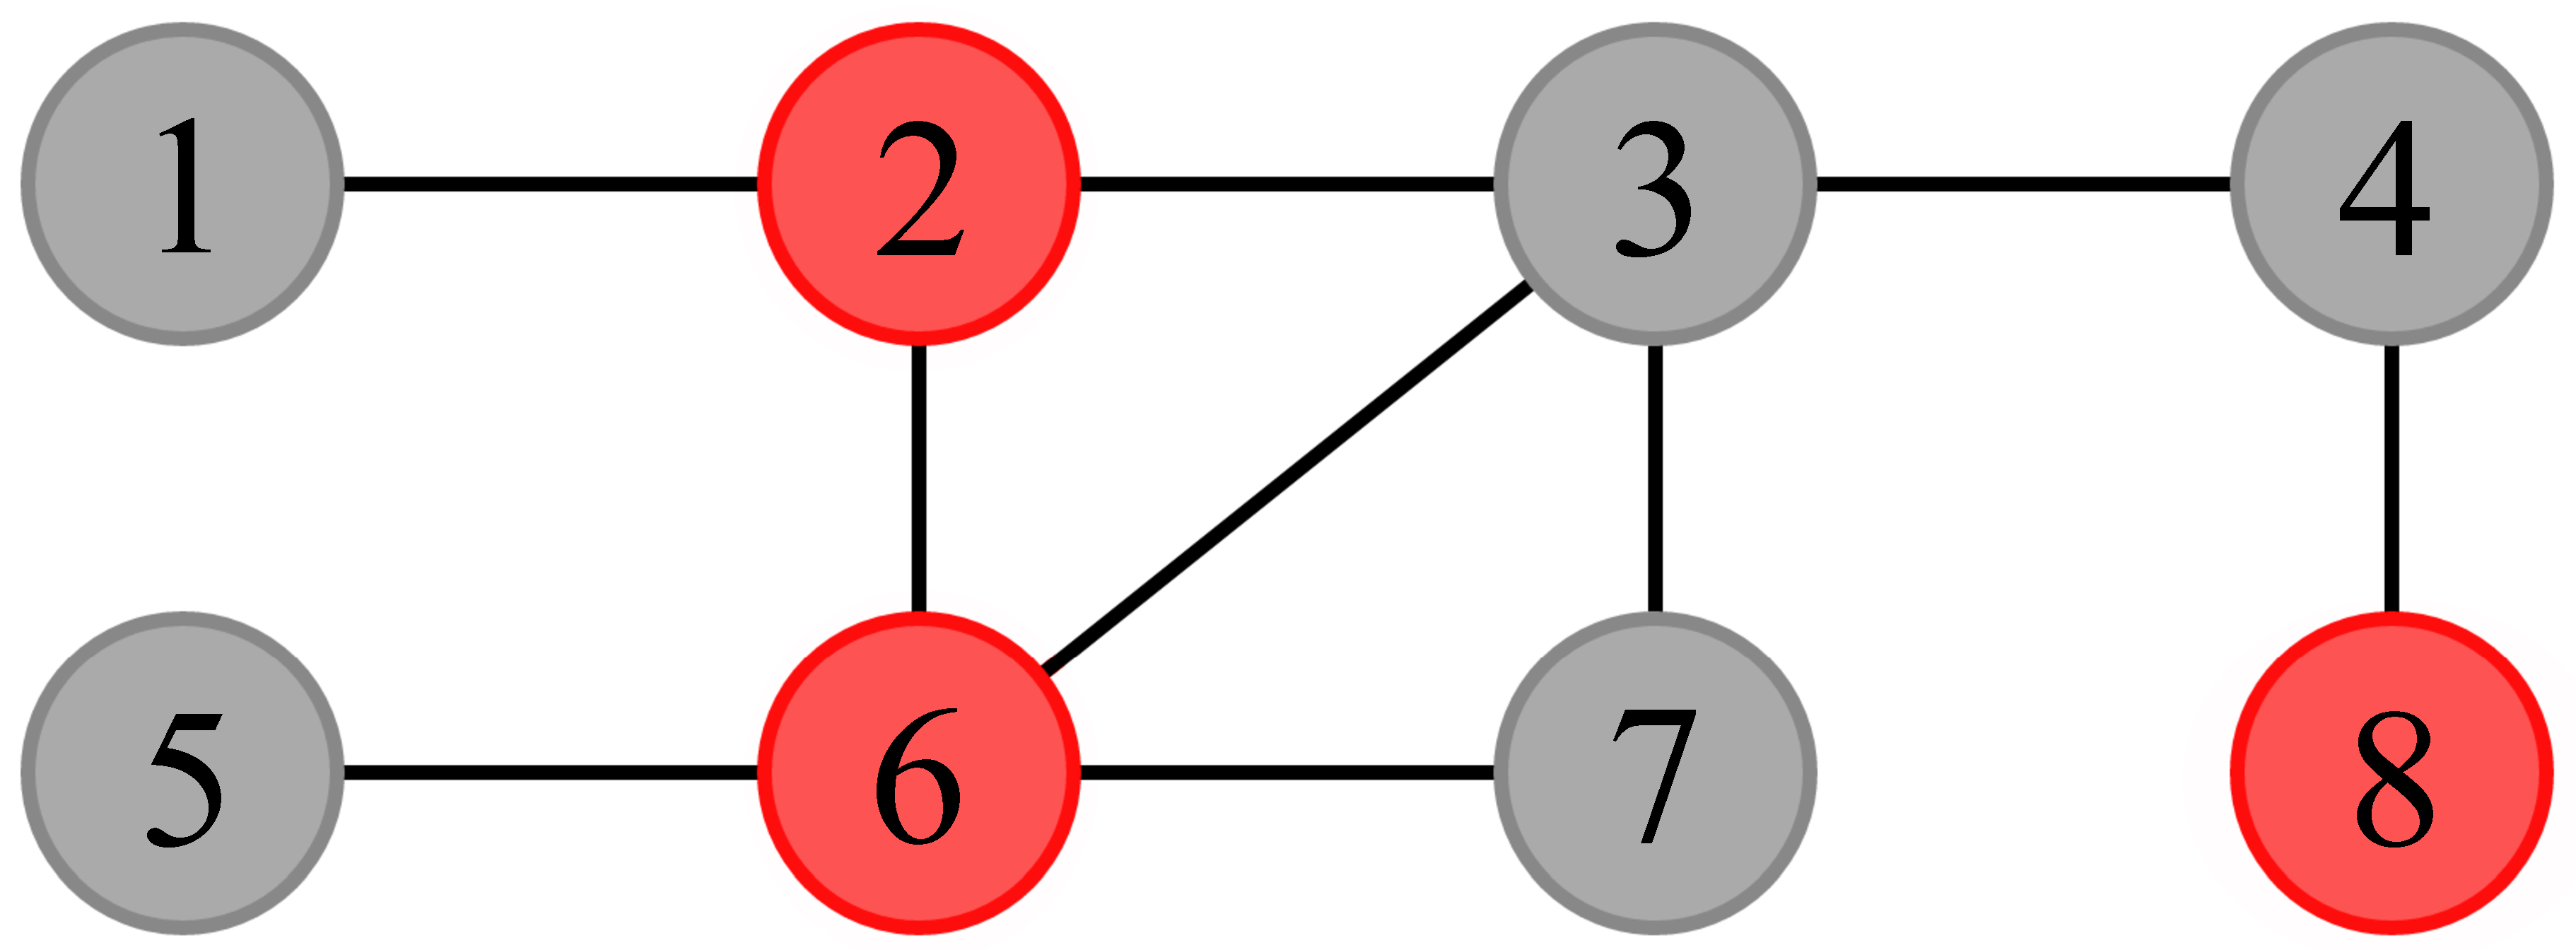
\includegraphics[width=6cm]{../figures/algorithm2-step1.pdf}
	\caption{A dominating set of $G_3$}\label{fig:algorithm2-step1}
\end{figure}

We assign our dominating set $\{2,6,8\}$ to $D$. Since $V \setminus D \neq \emptyset$, we enter the \emph{for all} loop in line 2. Here, we iterate through all vertices in $V \setminus D$. For each vertex $v \in V \setminus D$, we will pick another vertex in $D$ that is connected to $v$ by an edge. Then, we will contract the edge $\{u, v\}$ towards $u$. This means that we combine $u$ and $v$ together and update any edges to reflect the changes.

To illustrate this, we start the loop by picking a vertex $v$, say vertex 3. We pick vertex $u$ to be vertex 2 because $2 \in D$ and $\{2, 3\} \in E$. We contract the edge and show the resulting graph $G$ in Figure \ref{fig:algorithm2-step2}. By iterating over the rest of the vertices in $V \setminus D$, we obtain a graph that is itself a path from vertex 2 to vertex 6 to vertex 8. This graph, along with its proper vertex coloring, is shown in Figure \ref{fig:algorithm2-step3}. We can find a proper vertex coloring by any heuristic, such as a greedy algorithm, for the VCP.

\begin{figure}[h]
	\centering
	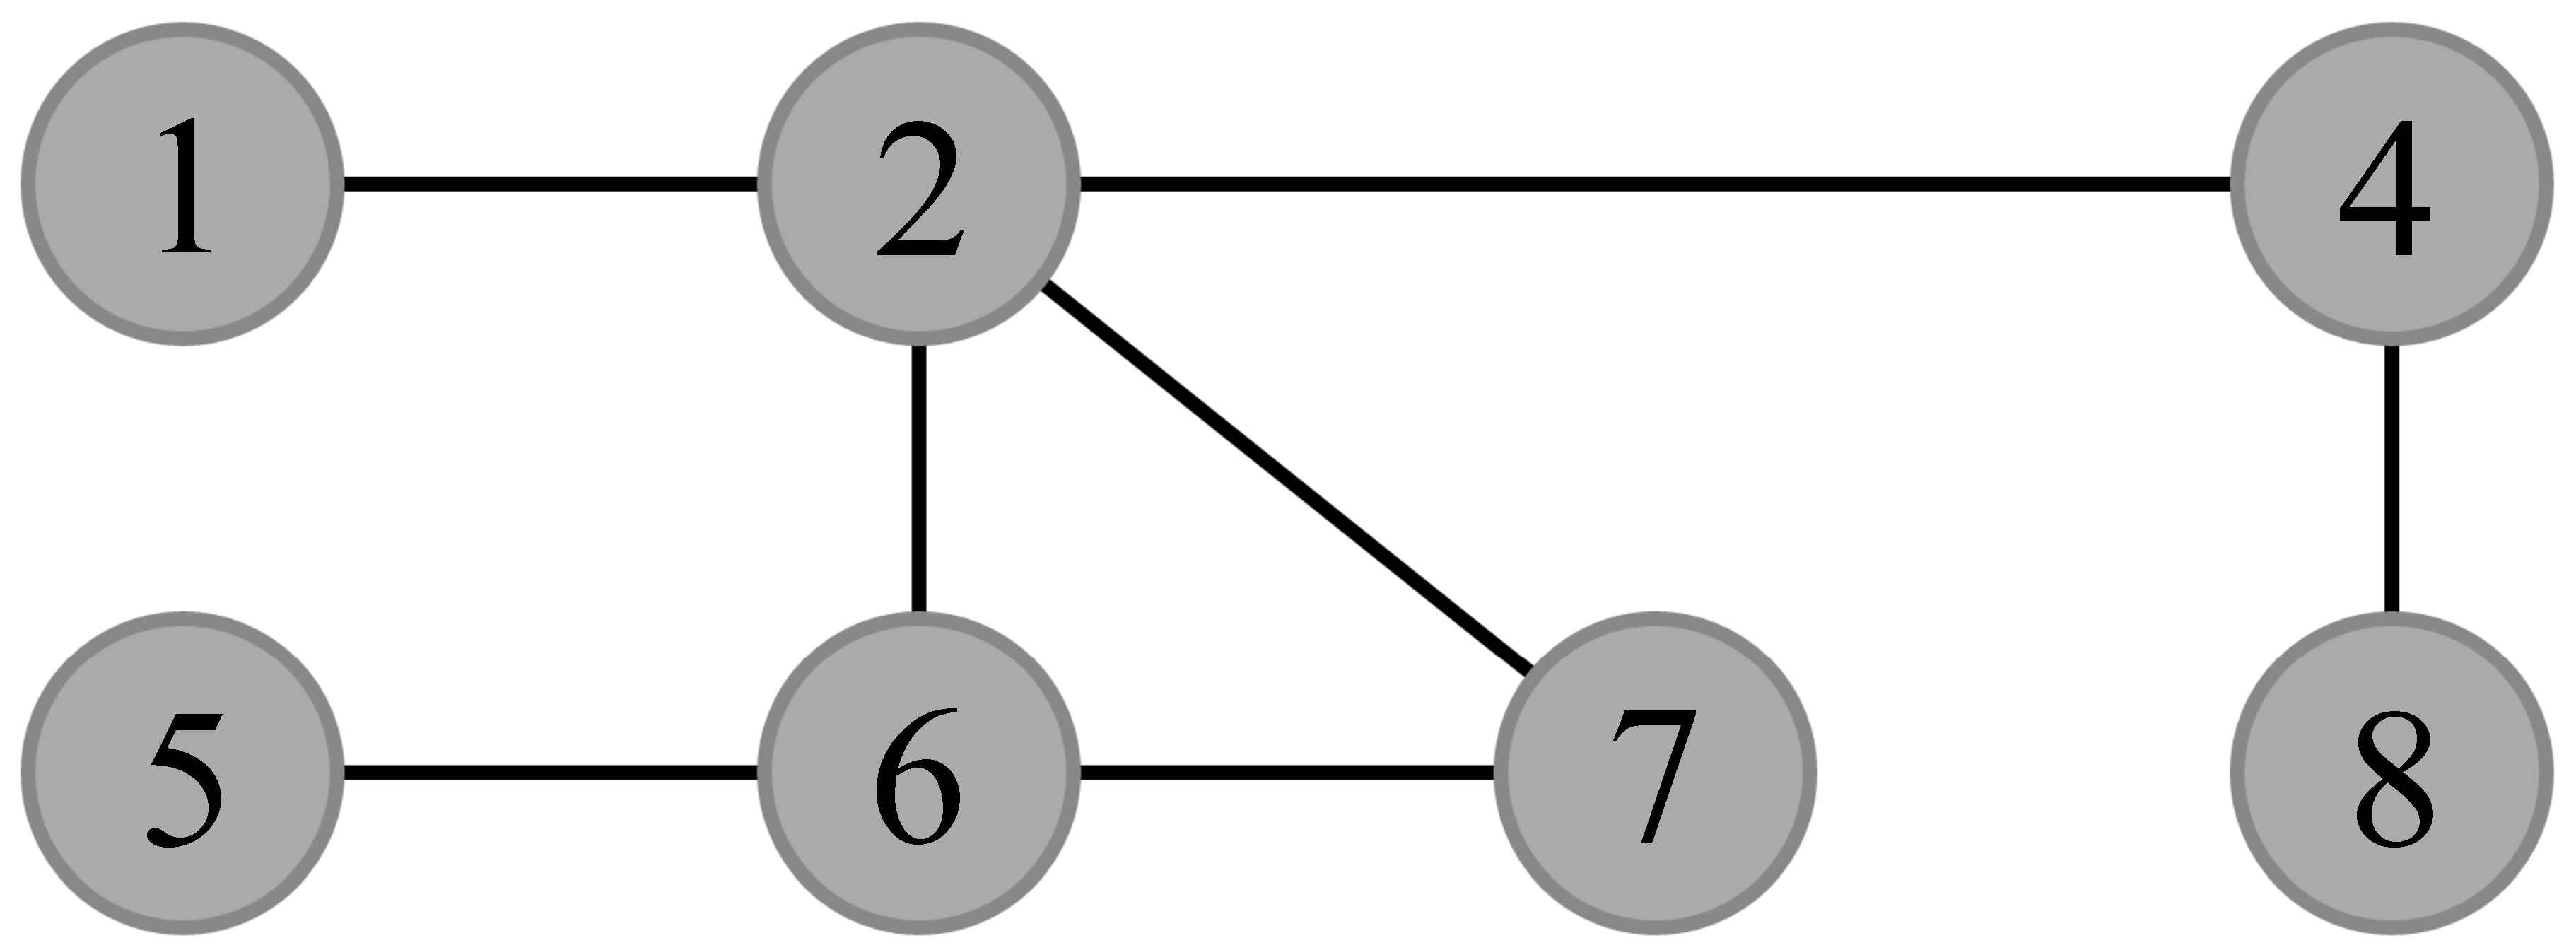
\includegraphics[width=6cm]{../figures/algorithm2-step2.pdf}
	\caption{The graph after the first \emph{for} loop}\label{fig:algorithm2-step2}
\end{figure}

Lastly, we color our original graph $G_3$ based on the proper vertex coloring we generated. We leave any nodes not in the graph $G$ uncolored when we color $G_3$. The coloring of $G_3$ is shown in Figure \ref{fig:algorithm2-step4}. It is clear that this has produced a conflict-free coloring.

\begin{figure}[h]
	\centering
	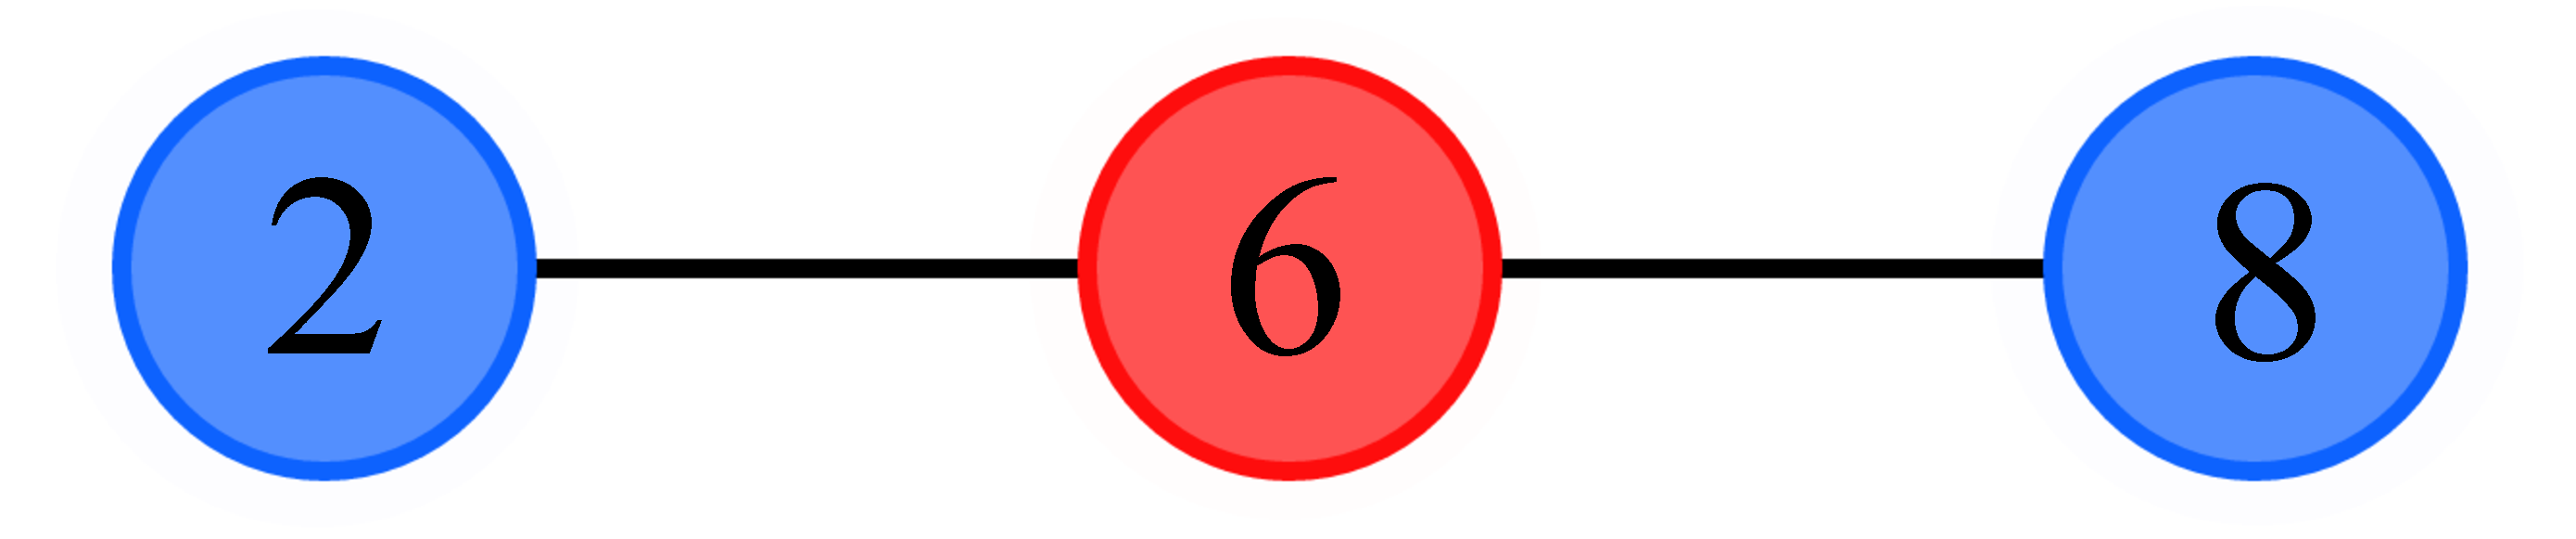
\includegraphics[width=5cm]{../figures/algorithm2-step3.pdf}
	\caption{The graph after lines 2-5}\label{fig:algorithm2-step3}
\end{figure}

Take note that this algorithm has produced fewer colored vertices than Algorithm \ref{alg:elimination}. We had 4 colored vertices based on that algorithm where here we have 3. This algorithm helps us prove theorems based on minimizing the number of colored vertices.

\begin{figure}[h]
	\centering
	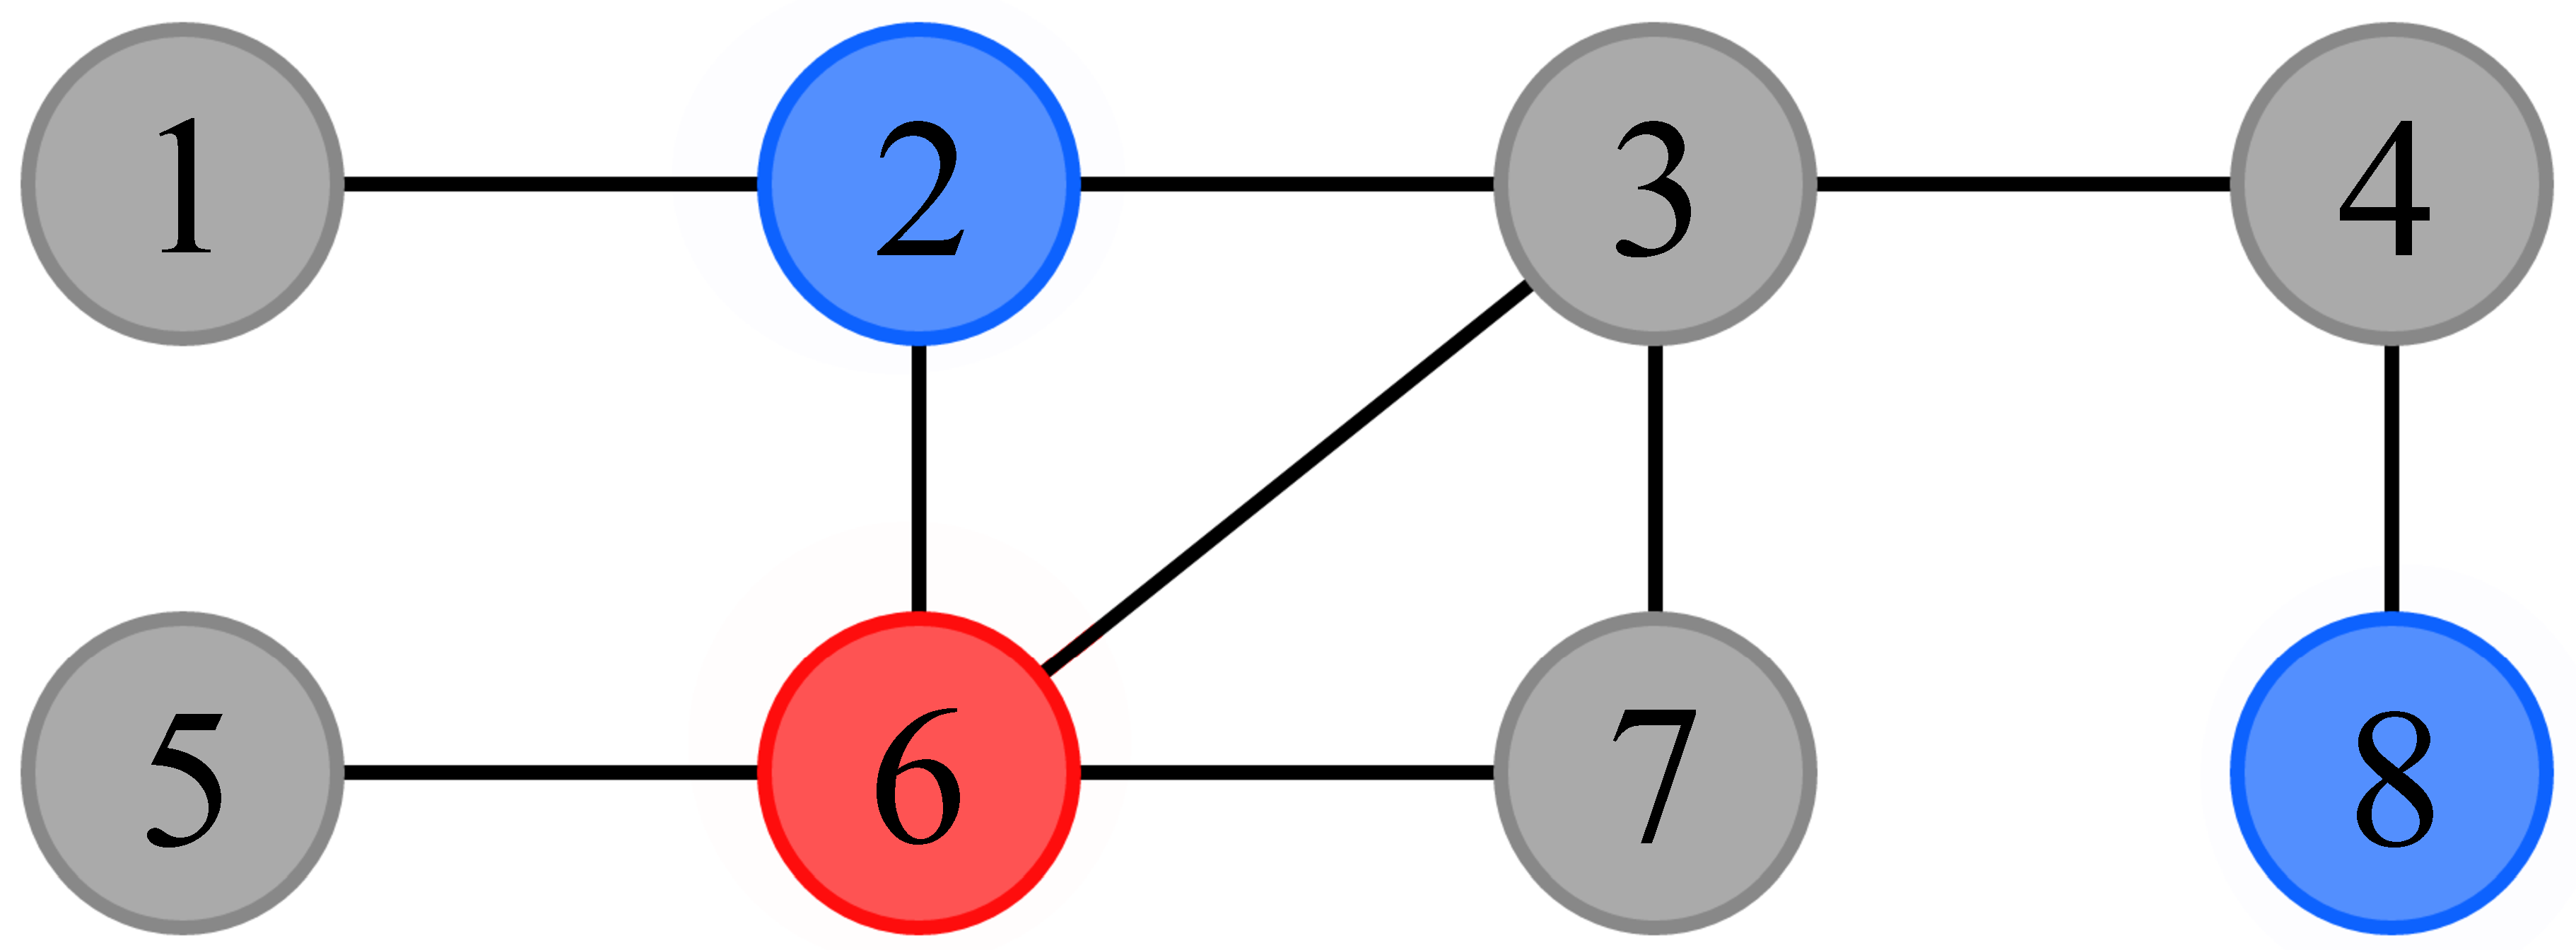
\includegraphics[width=6cm]{../figures/algorithm2-step4.pdf}
	\caption{$G_3$ with minimized colored vertices}\label{fig:algorithm2-step4}
\end{figure}

\vspace{-0.3cm}

\subsection{Minimizing Colored Vertices}
Abel et. al \cite{abel2017three} present results on minimizing colored vertices when conflict-free coloring planar graphs. They propose and prove Theorem \ref{thm:approximate-cfds} by using the polynomial-time algorithm described in Algorithm \ref{alg:cf-dominating}.

Because the planar minimum dominating set problem is NP-hard \cite{garey2002computers}, we know that the conflict-free dominating set problem is NP-hard because we aim to find a dominating set. It follows that the corresponding decision problem, the k-conflict-free dominating set problem, is NP-complete.

\begin{theorem} \label{thm:approximate-cfds}
For $k \geq 4$, the k-conflict-free dominating set problem is NP-complete and $\gamma_{CF}^k(G) = \gamma(G)$ for a planar graph $G$. Also, there exists a PTAS for estimating $\gamma_{CF}^k(G)$.
\end{theorem}

We get a PTAS for the conflict-free domination number by applying Algorithm \ref{alg:cf-dominating} and finding the dominating set using the PTAS defined by Baker and Hill \cite{baker1994approximation}. As the input graph $G$ is planar, the resulting graph $G'$ is also planar because $G'$ is a minor of $G$. Thus, it can be colored with 4 colors or less by Theorem \ref{thm:four}. We then color $G$ with the colors of $G'$, leaving any vertex in $G$ but not in $G'$ uncolored. This leaves us with a conflict-free coloring of $G$.

\vspace{-0.15cm}

\section{Conclusion}
\label{sec:conclusion}
We have presented some of the recent heuristics and findings on the conflict-free coloring problem. Although the CFCP is NP-hard and finding the minimum number colors needed requires inefficient brute force algorithms, there are heuristics to find good conflict-free colorings.

There are many applications of the CFCP that benefit from the recent research into conflict-free coloring. It is easier to minimize frequency assignment for wireless networks and design RFID networks. Current research focuses on finding bounds and properties on specific cases such as interval graphs, types of hypergraphs, and more \cite{cheilaris2014strong,smorodinsky2013conflict}.

There is also recent interest in variations of the CFCP such as requiring \emph{another} vertex (not the selected vertex) to be colored within the neighborhood of a selected vertex. This allows for applications such as guiding a specific robot to other locations (i.e. the robot and its destination would both be a distinct unique color). Relaxing the proper vertex coloring problem to satisfy new requirements leads to new heuristics that can effectively solve more real-world problems.

\vspace{-0.15cm}


\section{Acknowledgments}
Thanks to Peter Dolan, Elena Machkasova, Peh Ng, and Jeremy Eberhardt for their advice and feedback.

\vspace{-0.15cm}


\bibliographystyle{abbrv}
\bibliography{../references}


\end{document}
